\documentclass[11pt,a4paper]{article}
\usepackage[utf8]{inputenc}
\usepackage[T1]{fontenc}
\usepackage{geometry}
\usepackage{graphicx}
\usepackage{listings}
\usepackage{xcolor}
\usepackage{hyperref}
\usepackage{amsmath}
\usepackage{float}
\usepackage{booktabs}
\usepackage{multirow}
\usepackage{tikz}
\usetikzlibrary{shapes,arrows,positioning}

\geometry{margin=2.5cm}

% Code listing style
\lstset{
    language=C,
    basicstyle=\ttfamily\footnotesize,
    keywordstyle=\color{blue}\bfseries,
    commentstyle=\color{green!60!black},
    stringstyle=\color{red},
    numbers=left,
    numberstyle=\tiny\color{gray},
    stepnumber=1,
    numbersep=5pt,
    backgroundcolor=\color{gray!10},
    frame=single,
    breaklines=true,
    breakatwhitespace=true,
    tabsize=2,
    showspaces=false,
    showstringspaces=false,
    captionpos=b
}

\title{STM32F407 Telemetry System\\Complete Technical Documentation}
\author{Embedded Systems Project}
\date{\today}

\begin{document}

\maketitle
\tableofcontents
\newpage

\section{Project Overview}

\subsection{Introduction}
This document provides comprehensive technical documentation for a production-ready telemetry system based on the STM32F407VETx microcontroller. The system implements a fault-tolerant, scalable architecture using FreeRTOS for real-time task management, collecting data from multiple sensors (IMU, GPS) and transmitting telemetry via SPI.

\subsection{System Purpose}
The telemetry system is designed to:
\subsubsection{Why FreeRTOS?}
In a simple "Super Loop" architecture (typical Arduino sketch), the code runs top-to-bottom. If one function takes too long (like waiting for a sensor), everything else stops. 

With FreeRTOS, we split the code into independent \textbf{Tasks}. The \textbf{Scheduler} switches between them based on priority. If a high-priority task (like reading the IMU) needs to run, the scheduler pauses the low-priority task (like blinking an LED), runs the important one, and then resumes the other. This guarantees responsive timing.

\begin{figure}[H]
\centering
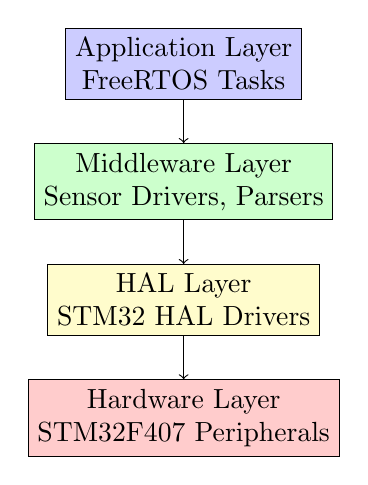
\begin{tikzpicture}[node distance=1.5cm, auto]
    \node [rectangle, draw, fill=blue!20, align=center] (app) {Application Layer\\FreeRTOS Tasks};
    \node [rectangle, draw, fill=green!20, below of=app, align=center] (mid) {Middleware Layer\\Sensor Drivers, Parsers};
    \node [rectangle, draw, fill=yellow!20, below of=mid, align=center] (hal) {HAL Layer\\STM32 HAL Drivers};
    \node [rectangle, draw, fill=red!20, below of=hal, align=center] (hw) {Hardware Layer\\STM32F407 Peripherals};
    
    \draw [->] (app) -- (mid);
    \draw [->] (mid) -- (hal);
    \draw [->] (hal) -- (hw);
\end{tikzpicture}
\caption{Software Architecture Layers}
\end{figure}

\subsection{Task Architecture}
The system implements 6 main FreeRTOS tasks with different priorities:

\begin{table}[H]
\centering
\begin{tabular}{@{}llll@{}}
\toprule
\textbf{Task} & \textbf{Priority} & \textbf{Stack Size} & \textbf{Function} \\
\midrule
IMU\_Task & High & 512 bytes & MPU6050 data acquisition \\
GPS\_Task & Above Normal & 512 bytes & GPS parsing and processing \\
Telemetry\_Task & Above Normal & 512 bytes & SPI telemetry transmission \\
UART\_Debug\_Task & Below Normal & 384 bytes & Debug output \\
LED\_Task & Low & 128 bytes & System heartbeat and monitoring \\
HEALTH\_Task & Low & 256 bytes & System health monitoring \\
\bottomrule
\end{tabular}
\caption{FreeRTOS Task Configuration}
\end{table}

\subsection{Data Flow}
\begin{figure}[H]
\centering
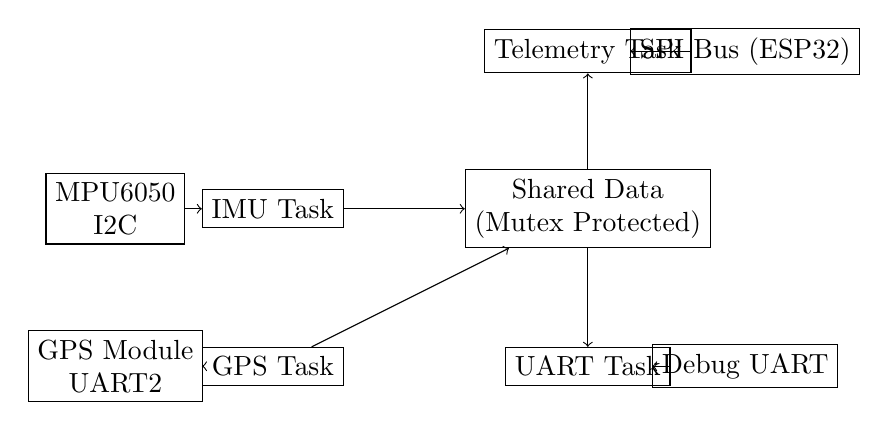
\begin{tikzpicture}[node distance=2cm, auto]
    \node [rectangle, draw, align=center] (imu) {MPU6050\\I2C};
    \node [rectangle, draw, right of=imu] (imutask) {IMU Task};
    \node [rectangle, draw, below of=imu, align=center] (gps) {GPS Module\\UART2};
    \node [rectangle, draw, right of=gps] (gpstask) {GPS Task};
    \node [rectangle, draw, right of=imutask, xshift=2cm, align=center] (shared) {Shared Data\\(Mutex Protected)};
    \node [rectangle, draw, above of=shared] (telmtask) {Telemetry Task};
    \node [rectangle, draw, below of=shared] (uarttask) {UART Task};
    \node [rectangle, draw, right of=telmtask] (spi) {SPI Bus (ESP32)};
    \node [rectangle, draw, right of=uarttask] (uart) {Debug UART};
    
    \draw [->] (imu) -- (imutask);
    \draw [->] (gps) -- (gpstask);
    \draw [->] (imutask) -- (shared);
    \draw [->] (gpstask) -- (shared);
    \draw [->] (shared) -- (telmtask);
    \draw [->] (shared) -- (uarttask);
    \draw [->] (telmtask) -- (spi);
    \draw [->] (uarttask) -- (uart);
\end{tikzpicture}
\caption{System Data Flow Diagram}
\end{figure}

\subsubsection{Data Protection (Mutexes)}
Since multiple tasks access the same data (e.g., IMU Task \textit{writes} data, Telemetry Task \textit{reads} it), we need protection. A \textbf{Mutex} (Mutual Exclusion) is like a key to a room.
\begin{itemize}
    \item When the IMU Task wants to update data, it "takes the key" (locks the mutex).
    \item If the Telemetry Task tries to read the data while the key is gone, it must wait.
    \item Once the IMU Task finishes, it "gives back the key" (unlocks), allowing the Telemetry Task to proceed.
\end{itemize}
This prevents "race conditions" where data might be read while it's being updated, leading to corrupted values.

\section{Hardware Configuration}

\subsection{Microcontroller}
\textbf{Device}: STM32F407VET6 \\
\textbf{Package}: LQFP100 \\
\textbf{Core}: ARM Cortex-M4F @ 72 MHz \\
\textbf{Flash}: 512 KB \\
\textbf{RAM}: 128 KB

\subsection{Clock Configuration}

The system uses an external 8 MHz crystal (HSE) with PLL to generate the system clock and USB clock.

\begin{table}[H]
\centering
\begin{tabular}{@{}ll@{}}
\toprule
\textbf{Parameter} & \textbf{Value} \\
\midrule
HSE Crystal & 8 MHz \\
PLL Configuration & PLLM=4, PLLN=72, PLLP=2, PLLQ=3 \\
VCO Frequency & 144 MHz \\
System Clock (HCLK) & 72 MHz \\
APB1 Clock & 36 MHz \\
APB2 Clock & 72 MHz \\
USB Clock & 48 MHz \\
\bottomrule
\end{tabular}
\caption{Clock Configuration}
\end{table}

\textbf{Clock Calculation}:
\begin{equation}
VCO = \frac{HSE}{PLLM} \times PLLN = \frac{8\text{ MHz}}{4} \times 72 = 144\text{ MHz}
\end{equation}

\begin{equation}
SYSCLK = \frac{VCO}{PLLP} = \frac{144\text{ MHz}}{2} = 72\text{ MHz}
\end{equation}

\begin{equation}
USB\_CLK = \frac{VCO}{PLLQ} = \frac{144\text{ MHz}}{3} = 48\text{ MHz}
\end{equation}

\subsection{Pin Assignment}

\subsubsection{I2C2 - MPU6050 IMU Sensor}

\begin{table}[H]
\centering
\begin{tabular}{@{}llp{8cm}@{}}
\toprule
\textbf{Pin} & \textbf{Function} & \textbf{Configuration} \\
\midrule
PB10 & I2C2\_SCL & AF4, Open-Drain, No Pull, 400 kHz \\
PB11 & I2C2\_SDA & AF4, Open-Drain, No Pull, 400 kHz \\
\bottomrule
\end{tabular}
\caption{I2C2 Pin Configuration}
\end{table}

\textbf{Important Notes}:
\begin{itemize}
    \item External pull-up resistors (4.7k$\Omega$) are \textbf{required} on both SCL and SDA lines
    \item Internal pull-ups are disabled for proper 400 kHz operation
    \item Device address: 0x68 (AD0=LOW) or 0x69 (AD0=HIGH)
\end{itemize}

\subsubsection{SPI2 - ESP32 Communication}

\begin{table}[H]
\centering
\begin{tabular}{@{}llp{8cm}@{}}
\toprule
\textbf{Pin} & \textbf{Function} & \textbf{Configuration} \\
\midrule
PC2 & SPI2\_MISO & AF5, Push-Pull, Master In Slave Out \\
PC3 & SPI2\_MOSI & AF5, Push-Pull, Master Out Slave In \\
PB13 & SPI2\_SCK & AF5, Push-Pull, Serial Clock \\
PB12 & SPI2\_CS & GPIO Output, Push-Pull, Software Controlled (Active LOW) \\
\bottomrule
\end{tabular}
\caption{SPI2 Pin Configuration}
\end{table}

\textbf{SPI Configuration}:
\begin{itemize}
    \item Mode: Master
    \item Clock Polarity: Low (CPOL=0)
    \item Clock Phase: 1st Edge (CPHA=0)
    \item Data Size: 8-bit
    \item Baud Rate Prescaler: 16 (APB1/16 $\approx$ 2.25 MHz)
    \item Bit Order: MSB First
    \item CS (PB12) initialized HIGH (deselected), driven LOW during transmission
\end{itemize}

\subsubsection{USART2 - GPS Module}

\begin{table}[H]
\centering
\begin{tabular}{@{}llp{8cm}@{}}
\toprule
\textbf{Pin} & \textbf{Function} & \textbf{Configuration} \\
\midrule
PA2 & USART2\_TX & AF7, Push-Pull, Transmit to GPS \\
PA3 & USART2\_RX & AF7, Push-Pull, Receive from GPS (DMA enabled) \\
\bottomrule
\end{tabular}
\caption{USART2 Pin Configuration}
\end{table}

\textbf{UART Configuration}:
\begin{itemize}
    \item Baud Rate: 9600 bps
    \item Data Bits: 8
    \item Stop Bits: 1
    \item Parity: None
    \item Flow Control: None
    \item DMA: DMA1 Stream 5, Channel 4 (RX only, Circular mode with idle detection)
\end{itemize}

\subsubsection{USART3 - Debug UART}

\begin{table}[H]
\centering
\begin{tabular}{@{}llp{8cm}@{}}
\toprule
\textbf{Pin} & \textbf{Function} & \textbf{Configuration} \\
\midrule
PD8 & USART3\_TX & AF7, Push-Pull, Debug output \\
PD9 & USART3\_RX & AF7, Push-Pull, Debug input \\
\bottomrule
\end{tabular}
\caption{USART3 Pin Configuration}
\end{table}

\textbf{UART Configuration}:
\begin{itemize}
    \item Baud Rate: 115200 bps
    \item Data Bits: 8
    \item Stop Bits: 1
    \item Parity: None
    \item Flow Control: None
    \item Purpose: System debug messages and logging
\end{itemize}

\subsubsection{USB OTG FS - Virtual COM Port}

\begin{table}[H]
\centering
\begin{tabular}{@{}llp{8cm}@{}}
\toprule
\textbf{Pin} & \textbf{Function} & \textbf{Configuration} \\
\midrule
PA11 & USB\_DM & AF10, USB OTG FS Data Minus \\
PA12 & USB\_DP & AF10, USB OTG FS Data Plus \\
\bottomrule
\end{tabular}
\caption{USB Pin Configuration}
\end{table}

\textbf{USB Configuration}:
\begin{itemize}
    \item Device Class: CDC (Communications Device Class)
    \item Function: Virtual COM Port
    \item Speed: Full Speed (12 Mbps)
    \item PA12 is temporarily driven LOW during initialization to force USB re-enumeration
\end{itemize}

\subsubsection{GPIO - LEDs and Indicators}

\begin{table}[H]
\centering
\begin{tabular}{@{}llp{8cm}@{}}
\toprule
\textbf{Pin} & \textbf{Function} & \textbf{Purpose} \\
\midrule
PD12 & Status LED & System status indicator (Output, Push-Pull) \\
PA6 & Error LED & Error indication (Output, Push-Pull) \\
PA7 & Error LED & Error indication (Output, Push-Pull) \\
\bottomrule
\end{tabular}
\caption{GPIO Pin Configuration}
\end{table}

\textbf{LED Behavior}:
\begin{itemize}
    \item \textbf{Normal Operation}: PD12 blinks 5 times during startup (200ms on/off)
    \item \textbf{Error Handler}: All LEDs toggle rapidly ($\approx$100ms) indicating fatal error
\end{itemize}

\subsection{Complete Pin Summary}

\begin{table}[H]
\centering
\begin{tabular}{@{}lllp{5cm}@{}}
\toprule
\textbf{Peripheral} & \textbf{Pins} & \textbf{Alt Function} & \textbf{Purpose} \\
\midrule
I2C2 & PB10, PB11 & AF4 & MPU6050 IMU \\
SPI2 & PC2, PC3, PB13, PB12 & AF5 + GPIO & ESP32 Communication \\
USART2 & PA2, PA3 & AF7 & GPS Module (DMA) \\
USART3 & PD8, PD9 & AF7 & Debug UART \\
USB OTG FS & PA11, PA12 & AF10 & Virtual COM Port \\
GPIO & PD12, PA6, PA7 & - & Status and Error LEDs \\
\bottomrule
\end{tabular}
\caption{Complete Pin Assignment Summary}
\end{table}

\begin{verbatim}
STM32           ESP32
PC3 (MOSI) ---> MISO (ESP32 SPI Slave)
PC2 (MISO) <--- MOSI (ESP32 SPI Slave)
PB13 (SCK) ---> SCK
PB12 (CS)  ---> CS
GND        ---> GND
\end{verbatim}

\subsubsection{GPS Module Connection}
\begin{verbatim}
STM32           GPS Module
PA2 (TX)   ---> RX
PA3 (RX)   <--- TX
3.3V/5V    ---> VCC (check GPS module voltage)
GND        ---> GND
\end{verbatim}

\subsubsection{Debug UART Connection}
\begin{verbatim}
STM32           USB-to-TTL Adapter
PD8 (TX)   ---> RX
PD9 (RX)   <--- TX
GND        ---> GND
\end{verbatim}

\subsection{Power Requirements}

\begin{table}[H]
\centering
\begin{tabular}{@{}ll@{}}
\toprule
\textbf{Pin} & \textbf{Function} \\
\midrule
VDD & Power Supply (3.3V nominal, multiple pins) \\
VSS & Ground (multiple pins) \\
VDDA & Analog Power (3.3V for ADC and analog circuits) \\
VSSA & Analog Ground \\
VBAT & Battery Backup (RTC and backup registers, optional) \\
\bottomrule
\end{tabular}
\caption{Power Pin Configuration}
\end{table}

\textbf{Important Power Notes}:
\begin{itemize}
    \item All VDD and VSS pins must be properly connected
    \item Use decoupling capacitors (100nF) close to each VDD pin
    \item Separate analog and digital grounds at single point
\end{itemize}

\subsection{Configuration Files}

Pin configurations are defined in the following source files:
\begin{itemize}
    \item \texttt{Core/Src/main.c}: System clock configuration and USB re-enumeration
    \item \texttt{Core/Src/gpio.c}: GPIO initialization (LEDs, SPI CS)
    \item \texttt{Core/Src/i2c.c}: I2C2 peripheral configuration
    \item \texttt{Core/Src/spi.c}: SPI2 peripheral configuration
    \item \texttt{Core/Src/usart.c}: USART2/3 configuration and DMA setup
\end{itemize}

\section{Detailed Task Implementation}

\subsection{IMU Task}
\textbf{File}: \texttt{Src/freertos.c}, function \texttt{StartIMU\_Task()}

\subsubsection{Purpose}
The IMU task is responsible for:
\begin{itemize}
    \item Initializing the MPU6050 sensor via I2C
    \item Reading accelerometer and gyroscope data at 10 Hz
    \item Calculating pitch, roll, and yaw angles
    \item Updating shared telemetry data with mutex protection
    \item Handling sensor failures gracefully
\end{itemize}

\subsubsection{Implementation Details}
The task implements retry logic for initialization and graceful degradation:

\begin{lstlisting}[caption=IMU Task Initialization with Retries, label=lst:imutask]
void StartIMU_Task(void const * argument)
{
  /* Register with task watchdog */
  TaskWatchdog_Register("IMU_Task");
  
  HAL_StatusTypeDef imu_init_status = HAL_ERROR;
  uint8_t init_retry_count = 0;
  const uint8_t MAX_INIT_RETRIES = ERROR_RECOVERY_RETRIES;  // 3 retries
  
  /* Try initialization with retries */
  while (imu_init_status != HAL_OK && init_retry_count < MAX_INIT_RETRIES) {
    if (osMutexWait(MUTEX_I2CHandle, pdMS_TO_TICKS(100)) == osOK) {
      imu_init_status = MPU6050_Init(&hi2c2);
      osMutexRelease(MUTEX_I2CHandle);
    }
    
    if (imu_init_status != HAL_OK) {
      init_retry_count++;
      if (init_retry_count < MAX_INIT_RETRIES) {
        osDelay(500);  // Wait before retry
      }
    }
  }
  
  /* If initialization fails, continue with graceful degradation */
  if (imu_init_status != HAL_OK) {
    // System continues, outputs zeros for IMU data
  }
}
\end{lstlisting}

\subsubsection{Complementary Filter for Angle Estimation}
The IMU task uses a \textbf{complementary filter} to combine accelerometer and gyroscope data for accurate angle estimation. This is a significant improvement over simple angle calculations.

\paragraph{The Problem with Individual Sensors}
\begin{itemize}
    \item \textbf{Accelerometer}: Provides absolute orientation relative to gravity (no drift), but is noisy and affected by vibrations and linear acceleration
    \item \textbf{Gyroscope}: Provides smooth, high-frequency rotation data, but drifts over time (accumulates error)
    \item \textbf{Simple integration}: Using only gyroscope causes drift; using only accelerometer causes noise
\end{itemize}

\paragraph{The Solution: Complementary Filter}
The complementary filter combines both sensors, using each where it performs best:
\begin{itemize}
    \item \textbf{Low frequencies} (slow changes): Trust accelerometer (corrects drift)
    \item \textbf{High frequencies} (fast changes): Trust gyroscope (smooth response)
\end{itemize}

\paragraph{Mathematical Foundation}
The complementary filter uses a weighted average:

\begin{equation}
\theta_{filtered} = \alpha \cdot \theta_{gyro} + (1 - \alpha) \cdot \theta_{accel}
\end{equation}

Where:
\begin{itemize}
    \item $\theta_{filtered}$ = Final filtered angle (pitch, roll, or yaw)
    \item $\theta_{gyro}$ = Angle from gyroscope integration
    \item $\theta_{accel}$ = Angle calculated from accelerometer
    \item $\alpha$ = Filter coefficient (0 to 1), typically 0.95-0.99
\end{itemize}

\paragraph{Filter Coefficient ($\alpha$)}
The coefficient $\alpha$ determines the balance:
\begin{itemize}
    \item \textbf{High $\alpha$ (0.98)}: More trust in gyroscope
    \begin{itemize}
        \item Smoother output (less noise)
        \item Better response to fast movements
        \item More drift over time (needs periodic correction)
    \end{itemize}
    \item \textbf{Low $\alpha$ (0.90)}: More trust in accelerometer
    \begin{itemize}
        \item Less drift (better long-term accuracy)
        \item More noise in output
        \item Slower response to movements
    \end{itemize}
\end{itemize}

In this system, $\alpha = 0.98$ is used, providing 98\% weight to gyroscope and 2\% to accelerometer for drift correction.

\paragraph{Gyroscope Integration}
The gyroscope provides angular \textit{rate} (degrees per second), which must be integrated to get angle:

\begin{equation}
\theta_{gyro}(t) = \theta_{gyro}(t-1) + \omega \cdot \Delta t
\end{equation}

Where:
\begin{itemize}
    \item $\theta_{gyro}(t)$ = Current gyroscope angle
    \item $\theta_{gyro}(t-1)$ = Previous gyroscope angle
    \item $\omega$ = Angular rate from gyroscope (deg/s)
    \item $\Delta t$ = Time step (seconds)
\end{itemize}

\paragraph{Accelerometer Angle Calculation}
For pitch and roll, angles are calculated from accelerometer using trigonometry:

\begin{equation}
\text{Pitch} = \arctan2\left(\frac{a_x}{\sqrt{a_y^2 + a_z^2}}\right) \times \frac{180}{\pi}
\end{equation}

\begin{equation}
\text{Roll} = \arctan2\left(\frac{a_y}{\sqrt{a_x^2 + a_z^2}}\right) \times \frac{180}{\pi}
\end{equation}

Where $a_x$, $a_y$, $a_z$ are accelerometer readings in m/s².

\textbf{Why these formulas?} The accelerometer measures gravity (9.8 m/s²) along each axis. When the device tilts, gravity components change. Using $\arctan2$ (two-argument arctangent) provides correct angle in all quadrants (-180° to +180°).

\paragraph{Yaw Limitation}
Yaw (rotation around vertical axis) cannot be determined from accelerometer alone because gravity doesn't change with yaw rotation. Therefore:
\begin{itemize}
    \item Yaw uses only gyroscope integration
    \item Will drift over time
    \item For accurate yaw, a magnetometer is needed (future enhancement)
\end{itemize}

\paragraph{Implementation}
\begin{lstlisting}[caption=Complementary Filter Implementation, label=lst:complementary]
/* Update complementary filter with new sensor data */
static TickType_t last_filter_update = 0;
TickType_t current_time = xTaskGetTickCount();
float dt = (current_time - last_filter_update) / configTICK_RATE_HZ;

/* Update filter - combines accel and gyro */
ComplementaryFilter_Update(&imu_filter,
                           local_imu.ax, local_imu.ay, local_imu.az,  // Accel
                           local_imu.gx, local_imu.gy, local_imu.gz,  // Gyro
                           local_imu.gx, local_imu.gy, local_imu.gz,  // Gyro
                           dt);  // Time delta

/* Update Kalman filter with WORLD frame acceleration (removing gravity) */
if (osMutexWait(kalmanMutexHandle, pdMS_TO_TICKS(10)) == osOK) {
    float wx, wy, wz;
    /* Helper to rotate IMU to World Frame using current Pitch/Roll/Yaw */
    imu_to_world(local_imu.ax, local_imu.ay, local_imu.az, 
                 local_imu.pitch, local_imu.roll, local_imu.yaw, 
                 &wx, &wy, &wz);
                 
    KalmanVelocity_UpdateIMU(&velocity_filter, wx, wy, wz - 9.8f, dt);
    osMutexRelease(kalmanMutexHandle);
}

/* Get filtered angles */
local_imu.pitch = ComplementaryFilter_GetPitch(&imu_filter);
local_imu.roll = ComplementaryFilter_GetRoll(&imu_filter);
local_imu.yaw = ComplementaryFilter_GetYaw(&imu_filter);
\end{lstlisting}

\textbf{File}: \texttt{Src/complementary\_filter.c}, function \texttt{ComplementaryFilter\_Update()}

\paragraph{Filter Initialization}
The filter is initialized once at system startup:

\begin{lstlisting}[caption=Complementary Filter Initialization, label=lst:compinit]
ComplementaryFilter_Init(&imu_filter, 0.98f);  // Alpha = 0.98
\end{lstlisting}

This sets the filter coefficient to 0.98, meaning 98\% weight on gyroscope and 2\% on accelerometer.

\subsection{Kalman Velocity Filter}
\textbf{File}: \texttt{Src/kalman\_velocity.c}

\subsubsection{Purpose}
The Kalman Velocity Filter fuses data from the IMU (accelerometer) and GPS to provide a robust, high-frequency velocity estimate.

\subsubsection{Why Kalman Filter?}
\begin{itemize}
    \item \textbf{IMU Integration}: Integrating accelerometer data gives high-frequency velocity updates but drifts rapidly due to sensor noise and bias.
    \item \textbf{GPS Data}: Provides accurate absolute velocity but at a slow rate (1-10 Hz) and with significant latency.
    \item \textbf{Fusion}: The Kalman filter uses the IMU for the "Prediction" step (fast updates) and GPS for the "Correction" step (correcting drift), providing the best of both worlds.
\end{itemize}

\subsubsection{Implementation Details}
The filter tracks 2D velocity ($v_x, v_y$).

\paragraph{Prediction Step (IMU)}
\begin{equation}
v_{new} = v_{old} + a_{world} \cdot \Delta t
\end{equation}
\begin{equation}
P_{new} = P_{old} + Q
\end{equation}
Where $Q$ is the process noise (accelerometer uncertainty).

\paragraph{Correction Step (GPS)}
\begin{equation}
K = \frac{P_{pred}}{P_{pred} + R}
\end{equation}
\begin{equation}
v_{est} = v_{pred} + K \cdot (v_{gps} - v_{pred})
\end{equation}
\begin{equation}
P_{est} = (1 - K) \cdot P_{pred}
\end{equation}
Where $R$ is the measurement noise (GPS uncertainty).

\paragraph{Zero Velocity Update (ZUPT)}
To prevent drift when the vehicle is stationary, a "Zero Velocity Clamp" is implemented. If the GPS reports a speed less than 0.5 m/s, the filter forces the velocity state to zero. This is crucial for preventing "phantom movement" while parked.

\begin{lstlisting}[caption=Kalman Filter ZUPT Logic, label=lst:kalmanzupt]
/* ZUPT: Zero Velocity Update when almost stationary */
if (parsed_gps.speed_ms < 0.5f) {
    KalmanVelocity_Reset(&velocity_filter);
} else {
    KalmanVelocity_UpdateGPS(&velocity_filter, vx, vy, parsed_gps.fix);
}
\end{lstlisting}

\subsection{GPS Task}
\textbf{File}: \texttt{Src/freertos.c}, function \texttt{StartGPS\_Task()}

\subsubsection{Purpose}
The GPS task processes NMEA sentences received via DMA and extracts position data.

\subsubsection{Data Reception}
GPS data is received using DMA with idle detection:

\begin{lstlisting}[caption=GPS DMA Reception Setup, label=lst:gpsdma]
// In MX_FREERTOS_Init():
HAL_UARTEx_ReceiveToIdle_DMA(&huart2, gps_rx_buf, GPS_RX_BUF_LEN);
__HAL_DMA_DISABLE_IT(&hdma_usart2_rx, DMA_IT_HT);  // Disable half-transfer
\end{lstlisting}

When DMA receives data, it triggers an interrupt that writes to a FreeRTOS stream buffer:

\begin{lstlisting}[caption=GPS DMA Callback, label=lst:gpscallback]
void HAL_UARTEx_RxEventCallback(UART_HandleTypeDef *huart, uint16_t Size)
{
  if (huart->Instance == USART2) {
    BaseType_t xHigherPriorityTaskWoken = pdFALSE;
    xStreamBufferSendFromISR(SB_GPS, gps_rx_buf, Size, &xHigherPriorityTaskWoken);
    portYIELD_FROM_ISR(xHigherPriorityTaskWoken);
    
    // Restart DMA reception
    HAL_UARTEx_ReceiveToIdle_DMA(&huart2, gps_rx_buf, GPS_RX_BUF_LEN);
  }
}
\end{lstlisting}

\textbf{Why DMA?} DMA allows non-blocking data reception, preventing task delays and ensuring real-time performance. The stream buffer provides thread-safe communication between ISR and task.

\subsubsection{NMEA Parsing}
The task processes NMEA sentences character-by-character:

\begin{lstlisting}[caption=GPS NMEA Parsing, label=lst:gpsparse]
void StartGPS_Task(void const * argument)
{
  char line_buf[128];
  size_t line_len = 0;
  
  for(;;) {
    // Receive data from stream buffer
    size_t len = xStreamBufferReceive(SB_GPS, rx_buf, sizeof(rx_buf), 
                                       pdMS_TO_TICKS(100));
    
    if(len > 0) {
      // Process each character
      for(size_t i = 0; i < len; i++) {
        char c = rx_buf[i];
        
        if(c == '\n' || c == '\r') {
          if(line_len > 0) {
            // Parse complete NMEA sentence
            GPS_ParseBuffer((uint8_t*)line_buf, line_len, &parsed_gps);
            line_len = 0;
          }
        } else if(c >= 32 && c < 127) {
          // Valid character - add to line buffer
          if(line_len < sizeof(line_buf) - 1) {
            line_buf[line_len++] = c;
          }
        }
      }
    }
  }
      }
    }
  }
}
\end{lstlisting}

\subsubsection{GPS Velocity Calculation & Fusion}
When GPS position/speed is updated, it is fused into the Kalman Filter. Note the use of the \textbf{Mutex} to protect the shared filter state.

\begin{lstlisting}[caption=GPS Task with Kalman Fusion and ZUPT, label=lst:gpsfusion]
/* ... parsing logic above ... */

/* Calculate velocity components */
vx = parsed_gps.speed_ms * cosf(course_rad);
vy = parsed_gps.speed_ms * sinf(course_rad);

/* Update Kalman filter (correction step) */
if (osMutexWait(kalmanMutexHandle, pdMS_TO_TICKS(10)) == osOK) {
    /* ZUPT: Zero Velocity Update when almost stationary */
    if (parsed_gps.speed_ms < 0.5f) {
        KalmanVelocity_Reset(&velocity_filter);
    } else {
        KalmanVelocity_UpdateGPS(&velocity_filter, vx, vy, parsed_gps.fix);
    }
    osMutexRelease(kalmanMutexHandle);
}

/* Update shared data */
if (osMutexWait(MUTEX_TELEMETRYHandle, pdMS_TO_TICKS(50)) == osOK) {
    /* ... update position ... */
    
    /* Get filtered velocity from Kalman filter */
    if (osMutexWait(kalmanMutexHandle, pdMS_TO_TICKS(10)) == osOK) {
        KalmanVelocity_GetVelocity(&velocity_filter, 
                                 &gps_data.velocity_x,
                                 &gps_data.velocity_y, 
                                 NULL, 
                                 &gps_data.speed);
        osMutexRelease(kalmanMutexHandle);
    }
    
    osMutexRelease(MUTEX_TELEMETRYHandle);
}
\end{lstlisting}
When GPS position is updated, velocity is obtained directly from the NMEA RMC sentences, which provide speed (in knots) and course (heading in degrees).

\paragraph{Velocity Components}
The system converts the speed and course into North-South (X) and East-West (Y) components for the Kalman filter:

\begin{equation}
v_x = \text{Speed}_{m/s} \cdot \cos(\text{Course}_{rad}) \quad (\text{North Component})
\end{equation}

\begin{equation}
v_y = \text{Speed}_{m/s} \cdot \sin(\text{Course}_{rad}) \quad (\text{East Component})
\end{equation}

Where:
\begin{itemize}
    \item $\text{Speed}_{m/s}$ = Speed converted from knots ($1 \text{ knot} \approx 0.5144 \text{ m/s}$)
    \item $\text{Course}_{rad}$ = Heading in radians ($0^\circ = \text{North}, 90^\circ = \text{East}$)
\end{itemize}

This method provides instantaneous velocity data, which is far more accurate and less noisy than calculating derivatives from position changes.

\subsubsection{GPS Parsing Function}
\textbf{File}: \texttt{Src/gps.c}, function \texttt{GPS\_ParseBuffer()}

The parser extracts data from GPGGA sentences:

\begin{lstlisting}[caption=GPS NMEA Field Extraction, label=lst:gpsfields]
HAL_StatusTypeDef GPS_ParseBuffer(uint8_t *buf, size_t len, GPS_Data_t *out)
{
  // Parse NMEA sentence: $GPGGA,time,lat,N/S,lon,E/W,quality,...
  char *token = strtok((char*)buf, ",");
  int field = 0;
  
  while(token != NULL) {
    switch(field) {
      case 2:  // Latitude (DDMM.MMMM format)
        lat_nmea = atof(token);
        break;
      case 3:  // Latitude hemisphere (N/S)
        lat_hemi = token[0];
        break;
      case 4:  // Longitude (DDDMM.MMMM format)
        lon_nmea = atof(token);
        break;
      case 5:  // Longitude hemisphere (E/W)
        lon_hemi = token[0];
        break;
      case 6:  // Fix quality (0=invalid, 1=GPS, 2=DGPS)
        out->fix = atoi(token);
        break;
      case 9:  // Altitude
        out->altitude = atof(token);
        break;
    }
    token = strtok(NULL, ",");
    field++;
  }
  
  // Convert NMEA format to decimal degrees
  out->latitude = nmea_to_decimal(lat_nmea, lat_hemi);
  out->longitude = nmea_to_decimal(lon_nmea, lon_hemi);
}
\end{lstlisting}


\subsection{Health Monitoring Task}
\textbf{File}: \texttt{Src/freertos.c}, function \texttt{StartHealth\_Task()}

\subsubsection{Purpose}
The Health Task monitors the "heartbeat" of critical sensors (IMU and GPS). If a sensor stops updating its data (e.g., due to I2C hang or GPS disconnection), the Health Task flags it as "Stale" or "Error".

\subsubsection{Mechanism}
\begin{itemize}
    \item \textbf{Timestamps}: Every time the IMU or GPS task updates data, it records the current timestamp (`xTaskGetTickCount`).
    \item \textbf{Monitoring}: The Health Task wakes up every 500ms and checks the difference between `current_time` and the last update timestamp.
    \item \textbf{Thresholds}:
    \begin{itemize}
        \item IMU Stale: > 2000 ms (2 seconds)
        \item GPS Stale: > 5000 ms (5 seconds)
    \end{itemize}
\end{itemize}

\begin{lstlisting}[caption=Health Task Implementation, label=lst:healthtask]
void StartHealth_Task(void const * argument)
{
  TaskWatchdog_Register("Health_Task");
  
  for(;;) {
    /* Update health status */
    Health_Update();
    
    TaskWatchdog_Feed("Health_Task");
    osDelay(pdMS_TO_TICKS(1000 / HEALTH_TASK_FREQ_HZ));
  }
}

/* Inside Health_Update(): */
/* Health data is updated under its own mutex (health_mutex) */
/* IMPORTANT: sys_status is NOT written here to avoid a data
   race -- the IMU and Telemetry tasks own sys_status under
   MUTEX_TELEMETRYHandle. */
health_data.imu_healthy =
  ((current_time - health_data.last_imu_update) <= imu_stale_ticks) ? 1 : 0;
health_data.gps_healthy =
  ((current_time - health_data.last_gps_update) <= gps_stale_ticks) ? 1 : 0;
\end{lstlisting}

\textbf{Design Decision -- Separating Health from sys\_status}:
The Health task only updates its own \texttt{HealthData\_t} structure under \texttt{health\_mutex}.
The \texttt{sys\_status} global is owned by the IMU and Telemetry tasks, which already set
\texttt{sys\_status.imu\_ok} and \texttt{sys\_status.gps\_ok} under \texttt{MUTEX\_TELEMETRYHandle}.
Having the Health task also write \texttt{sys\_status} without holding the correct mutex would
create a data race on a shared global, so it was removed.

\subsection{UART Debug Task}
\textbf{File}: \texttt{Src/freertos.c}, function \texttt{StartUART\_Task()}

\subsubsection{Purpose}
The UART Debug Task provides human-readable telemetry output via UART3 at 2 Hz. This is useful for debugging, monitoring, and development.

\subsubsection{Output Format}
The task outputs formatted telemetry data including:
\begin{itemize}
    \item Filtered IMU angles (pitch, roll, yaw) from complementary filter
    \item GPS coordinates (latitude, longitude)
    \item Kalman filtered velocity (Vx, Vy, Speed)
    \item Sensor status (IMU OK/ERR, GPS OK/ERR)
\end{itemize}

\subsubsection{Implementation}
\begin{lstlisting}[caption=UART Debug Task, label=lst:uarttask]
void StartUART_Task(void const * argument)
{
  char msg[160];
  
  // Wait for system to settle
  osDelay(1000);
  
  for(;;) {
    // Get shared data with mutex protection
    float pitch_val, roll_val, yaw_val;
    double lat_val, lon_val;
    float velocity_x, velocity_y, velocity_speed;
    uint8_t imu_ok, gps_ok;
    
    if (osMutexWait(MUTEX_TELEMETRYHandle, osWaitForever) == osOK) {
      pitch_val = imu_data.pitch;  // Complementary filtered
      roll_val = imu_data.roll;     // Complementary filtered
      yaw_val = imu_data.yaw;       // Gyro integrated
      lat_val = gps_data.latitude;
      lon_val = gps_data.longitude;
      imu_ok = sys_status.imu_ok;
      gps_ok = sys_status.gps_ok;
      osMutexRelease(MUTEX_TELEMETRYHandle);
    }
    
    // Get velocity from Kalman filter
    KalmanVelocity_GetVelocity(&velocity_filter, 
                               &velocity_x, &velocity_y, NULL, &velocity_speed);
    
    // Format output string
    int len = sprintf(msg,
      "Pitch: %.2f Roll: %.2f Yaw: %.2f | Lat: %.5f Lon: %.5f | "
      "Vx: %.2f Vy: %.2f Speed: %.2f m/s | IMU:%s GPS:%s\r\n",
      pitch_val, roll_val, yaw_val,
      lat_val, lon_val,
      velocity_x, velocity_y, velocity_speed,
      imu_ok ? "OK" : "ERR",
      gps_ok ? "OK" : "ERR");
    
    // Non-blocking transmit
    if (len > 0 && huart3.gState == HAL_UART_STATE_READY) {
      HAL_UART_Transmit(&huart3, (uint8_t*)msg, len, 10);
    }
    
    osDelay(500);  // 2 Hz output rate
  }
}
\end{lstlisting}

\textbf{Why non-blocking UART?} Prevents the task from hanging if UART is busy, ensuring real-time performance and preventing system freezes.

\subsection{LED Task}
\textbf{File}: \texttt{Src/freertos.c}, function \texttt{StartLED\_Task()}

\subsubsection{Purpose}
The LED Task provides visual system status indication through GPIO PD12. It implements different blink patterns to indicate system health and task status.

\subsubsection{LED Patterns}
\begin{itemize}
    \item \textbf{Normal operation}: Slow blink (1 Hz) - indicates system is running
    \item \textbf{Dead tasks detected}: Rapid blink pattern - number of blinks indicates number of dead tasks
    \item \textbf{System error}: Continuous rapid blinking - indicates critical failure
\end{itemize}

\subsubsection{Implementation}
\begin{lstlisting}[caption=LED Task, label=lst:ledtask]
void StartLED_Task(void const * argument)
{
  TaskWatchdog_Register("LED_Task");
  
  for(;;) {
    // Check for dead tasks
    uint8_t dead_tasks = TaskWatchdog_GetDeadTaskCount();
    
    if (dead_tasks > 0) {
      // Rapid blink pattern to indicate dead tasks
      for (int i = 0; i < dead_tasks && i < 5; i++) {
        HAL_GPIO_TogglePin(GPIOD, GPIO_PIN_12);
        osDelay(100);
      }
      osDelay(1000);
    } else {
      // Normal operation: slow blink
      HAL_GPIO_TogglePin(GPIOD, GPIO_PIN_12);
      osDelay(500);  // 1 Hz blink rate
    }
    
    TaskWatchdog_Feed("LED_Task");
  }
}
\end{lstlisting}

\textbf{Why LED task?} Provides immediate visual feedback about system health without requiring UART connection. Useful for field deployment and quick diagnostics.

\subsection{Health Task}
\textbf{File}: \texttt{Src/health.c}, function \texttt{Health\_Task()}

\subsubsection{Purpose}
The Health Task monitors overall system health by tracking sensor update rates and detecting stale data. It provides system-level health status.

\subsubsection{Functionality}
\begin{itemize}
    \item Monitors IMU and GPS update rates
    \item Detects stale data (no updates for extended period)
    \item Updates system health status
    \item Provides health statistics
\end{itemize}

\subsubsection{Health Notifications}
Other tasks notify the health system when data is updated:
\begin{lstlisting}[caption=Health Notifications, label=lst:healthnotify]
// In IMU task, after successful read:
Health_NotifyIMUUpdated();

// In GPS task, after successful parse:
Health_NotifyGPSUpdated();
\end{lstlisting}

\textbf{Why separate health task?} Centralizes health monitoring logic, making it easier to add new health checks and maintain system diagnostics.

\subsection{Telemetry Task}
\textbf{File}: \texttt{Src/freertos.c}, function \texttt{StartTelemetry\_Task()}

\subsubsection{Purpose}
Transmits telemetry data via SPI bus to an ESP32. The task runs at 10 Hz and sends a structured packet containing IMU, GPS, and system status data.

\subsubsection{SPI Packet Structure (Current: 79 bytes)}
The system uses a fixed-length packet format for reliable parsing.
The packet was redesigned in February 2026 to add a boot timestamp (\texttt{t\_ms}),
a sequence counter (\texttt{seq}), raw sensor data, and satellite count.

\begin{table}[H]
\centering
\begin{tabular}{@{}llll@{}}
\toprule
\textbf{Byte Offset} & \textbf{Field} & \textbf{Type} & \textbf{Description} \\
\midrule
\multicolumn{4}{c}{\textbf{Header (3 bytes)}} \\
\midrule
0 & Start Byte & uint8 & Fixed 0xAA \\
1 & Packet Type & uint8 & 0x01 = Telemetry \\
2 & Payload Len & uint8 & 74 \\
\midrule
\multicolumn{4}{c}{\textbf{Basic Info (6 bytes)}} \\
\midrule
3--6 & t\_ms & uint32 & Boot timestamp (ms) \\
7--8 & seq & uint16 & Sequence counter \\
\midrule
\multicolumn{4}{c}{\textbf{Orientation (12 bytes)}} \\
\midrule
9--12 & Pitch & float & IMU Pitch (deg) \\
13--16 & Roll & float & IMU Roll (deg) \\
17--20 & Yaw & float & IMU Yaw (deg) \\
\midrule
\multicolumn{4}{c}{\textbf{Raw Accel (12 bytes)}} \\
\midrule
21--24 & ax & float & Accel X (m/s\textsuperscript{2}) \\
25--28 & ay & float & Accel Y (m/s\textsuperscript{2}) \\
29--32 & az & float & Accel Z (m/s\textsuperscript{2}) \\
\midrule
\multicolumn{4}{c}{\textbf{Raw Gyro (12 bytes)}} \\
\midrule
33--36 & gx & float & Gyro X (deg/s) \\
37--40 & gy & float & Gyro Y (deg/s) \\
41--44 & gz & float & Gyro Z (deg/s) \\
\midrule
\multicolumn{4}{c}{\textbf{GPS Speed (4 bytes)}} \\
\midrule
45--48 & speed & float & Ground speed (m/s) \\
\midrule
\multicolumn{4}{c}{\textbf{GPS Position (20 bytes)}} \\
\midrule
49--56 & latitude & double & Latitude (deg) \\
57--64 & longitude & double & Longitude (deg) \\
65--68 & altitude & float & Altitude (m) \\
\midrule
\multicolumn{4}{c}{\textbf{Status \& Quality (8 bytes)}} \\
\midrule
69 & imu\_ok & uint8 & IMU status (0/1) \\
70 & gps\_ok & uint8 & GPS status (0/1) \\
71 & fix & uint8 & GPS fix quality \\
72 & satellites & uint8 & Satellites tracked \\
73--76 & hdop & float & Horizontal DOP \\
\midrule
\multicolumn{4}{c}{\textbf{Footer (3 bytes)}} \\
\midrule
77 & Checksum & uint8 & XOR of bytes 0--76 \\
78 & End Byte & uint8 & Fixed 0x55 \\
\bottomrule
\end{tabular}
\caption{SPI Telemetry Packet Structure (79 bytes total)}
\end{table}

\textbf{Why this layout?}
\begin{itemize}
    \item \textbf{t\_ms}: Allows the receiver to compute inter-packet timing even if SPI jitters.
    \item \textbf{seq}: Lets the receiver detect dropped packets (gaps in the counter).
    \item \textbf{Raw accel/gyro}: Enables the receiver to run its own filtering or replay.
    \item \textbf{satellites}: Provides GPS quality feedback without parsing HDOP.
    \item \textbf{Checksum}: Simple XOR of the entire packet excluding the end byte ensures integrity with minimal CPU cost.
\end{itemize}

\subsubsection{SPI Configuration}
\textbf{Peripheral}: SPI2 \\
\textbf{Mode}: Master \\
\textbf{Pins}:
\begin{itemize}
    \item \textbf{SCK}: PB13
    \item \textbf{MISO}: PB14
    \item \textbf{MOSI}: PB15
    \item \textbf{CS}: PB12 (Software Controlled)
\end{itemize}

\subsubsection{Implementation}
The task constructs the packet and transmits it using blocking SPI with a short timeout.

\begin{lstlisting}[caption=Telemetry Task Implementation, label=lst:telmtask]
void StartTelemetry_Task(void const * argument)
{
  /* Wait for SPI to be ready */
  osDelay(100);
  
  uint8_t txData[32];
  TickType_t last_telemetry_send = 0;
  
  for(;;) {
    TickType_t now = xTaskGetTickCount();
    
    /* Send Telemetry at 10 Hz */
    if ((now - last_telemetry_send) >= pdMS_TO_TICKS(100)) {
      
      /* Get shared data with mutex protection */
      if (osMutexWait(MUTEX_TELEMETRYHandle, pdMS_TO_TICKS(50)) == osOK) {
        // Copy data...
        osMutexRelease(MUTEX_TELEMETRYHandle);
      }
      
      /* Prepare SPI Packet */
      txData[0] = 0xAA; /* Start Byte */
      txData[1] = 0x01; /* Type: Telemetry */
      txData[2] = 39;   /* Payload Length */
      
      // Copy float data using memcpy to avoid alignment issues
      memcpy(&txData[3], &pitch_val, 4);
      memcpy(&txData[7], &roll_val, 4);
      // ... copy other fields (Yaw, Speed, Lat, Lon, Alt) ...
      
      /* Calculate Checksum */
      uint8_t checksum = 0;
      for(int i=0; i<42; i++) {
        checksum ^= txData[i];
      }
      txData[42] = checksum;
      txData[43] = 0x55; /* End Byte */
      
      /* Transmit via SPI */
      HAL_GPIO_WritePin(GPIOB, GPIO_PIN_12, GPIO_PIN_RESET); // CS Low
      
      if (HAL_SPI_Transmit(&hspi2, txData, 29, 100) == HAL_OK) {
        spi_tx_success_count++;
      } else {
        spi_tx_error_count++;
      }
      
      HAL_GPIO_WritePin(GPIOB, GPIO_PIN_12, GPIO_PIN_SET); // CS High
      
      last_telemetry_send = now;
    }
    
    osDelay(10);
  }
}
\end{lstlisting}

\textbf{Why SPI Packet Structure?}
\begin{itemize}
    \item \textbf{Efficiency}: Fixed-length packets are easy to parse
    \item \textbf{Simplicity}: No need for complex ID filtering
    \item \textbf{Speed}: High-speed data transfer to ESP32
    \item \textbf{Integrity}: Checksum ensures data validity
\end{itemize}

\section{Communication Protocols}

\subsection{Protocol Analogies}
To understand how different parts of the system talk to each other, consider these analogies:

\begin{itemize}
    \item \textbf{I2C (Inter-Integrated Circuit)}: Like a \textbf{Conference Call}.
    \begin{itemize}
        \item There are two wires: Data (SDA) and Clock (SCL).
        \item The Master (STM32) calls out an address ("Hey MPU6050!").
        \item Only the device with that address responds.
        \item It's efficient for connecting many sensors to just two pins, but it's relatively slow.
    \end{itemize}
    
    \item \textbf{SPI (Serial Peripheral Interface)}: Like a \textbf{Direct Data Pipe}.
    \begin{itemize}
        \item Uses 4 wires: Clock (SCK), Data Out (MOSI), Data In (MISO), and Select (CS).
        \item It's much faster than I2C.
        \item The "Chip Select" (CS) line is like a dedicated switch. When pulled low, the device listens.
        \item We use this for Telemetry because we need to send data fast.
    \end{itemize}
    
    \item \textbf{UART (Universal Asynchronous Receiver-Transmitter)}: Like \textbf{Text Messaging}.
    \begin{itemize}
        \item No clock wire, just TX (Transmit) and RX (Receive).
        \item Both sides must agree on the speed (Baud Rate) beforehand.
        \item Good for simple text data (like GPS NMEA sentences or debug messages).
    \end{itemize}
\end{itemize}

\subsection{I2C Communication (MPU6050)}
\textbf{File}: \texttt{Src/mpu6050.c}

\subsubsection{Initialization}
\begin{lstlisting}[caption=MPU6050 Initialization (Robust), label=lst:mpuinit]
HAL_StatusTypeDef MPU6050_Init(I2C_HandleTypeDef *hi2c)
{
  uint8_t check;
  uint8_t mpu_addr = 0xD0;  // 0x68 << 1 (8-bit address)
  
  // 1. Software Reset (Critical for stability)
  // Write 0x80 to PWR_MGMT_1 to reset the device
  uint8_t data = 0x80;
  HAL_I2C_Mem_Write(hi2c, mpu_addr, 0x6B, I2C_MEMADD_SIZE_8BIT, &data, 1, 100);
  HAL_Delay(100); // Wait for reset
  
  // 2. Signal Path Reset
  // Write 0x07 to SIGNAL_PATH_RESET to clear analog/digital paths
  data = 0x07;
  HAL_I2C_Mem_Write(hi2c, mpu_addr, 0x68, I2C_MEMADD_SIZE_8BIT, &data, 1, 100);
  HAL_Delay(100);
  
  // 3. Wake up & Clock Config
  // Write 0x01 to PWR_MGMT_1: Wake up + Select PLL with X-axis gyro ref
  // This is much more stable than the internal 8MHz oscillator
  data = 0x01;
  HAL_I2C_Mem_Write(hi2c, mpu_addr, 0x6B, I2C_MEMADD_SIZE_8BIT, &data, 1, 100);
  HAL_Delay(50);
  
  // 4. Configure Filters and Ranges
  // DLPF (Digital Low Pass Filter) = 5Hz bandwidth
  data = 0x06;
  HAL_I2C_Mem_Write(hi2c, mpu_addr, 0x1A, I2C_MEMADD_SIZE_8BIT, &data, 1, 100);
  
  // Accelerometer: $\pm$8G range
  data = 0x10;
  HAL_I2C_Mem_Write(hi2c, mpu_addr, 0x1C, I2C_MEMADD_SIZE_8BIT, &data, 1, 100);
  
  // Gyroscope: $\pm$500$^\circ$/s range
  data = 0x08;
  HAL_I2C_Mem_Write(hi2c, mpu_addr, 0x1B, I2C_MEMADD_SIZE_8BIT, &data, 1, 100);
  
  return HAL_OK;
}
\end{lstlisting}

\subsubsection{Data Reading}
\begin{lstlisting}[caption=MPU6050 Data Reading, label=lst:mpuread]
HAL_StatusTypeDef MPU6050_Read_All(I2C_HandleTypeDef *hi2c, IMU_Data_t *DataStruct)
{
  uint8_t data[14];  // Accel (6) + Temp (2) + Gyro (6)
  
  // Read all registers in one transaction (0x3B to 0x48)
  HAL_StatusTypeDef res = HAL_I2C_Mem_Read(hi2c, mpu6050_active_addr, 0x3B,
                                           I2C_MEMADD_SIZE_8BIT, data, 14, 50);
  
  if (res != HAL_OK) {
    /* Only zero sensor readings, NOT calibration offsets.
       A memset of the entire struct would wipe the offsets
       computed during the 1-second boot calibration, causing
       all future readings to be uncalibrated until reboot. */
    DataStruct->ax = 0; DataStruct->ay = 0; DataStruct->az = 0;
    DataStruct->gx = 0; DataStruct->gy = 0; DataStruct->gz = 0;
    return HAL_ERROR;
  }
  
  // Parse 16-bit values (big-endian)
  int16_t raw_ax = (data[0] << 8) | data[1];
  int16_t raw_ay = (data[2] << 8) | data[3];
  int16_t raw_az = (data[4] << 8) | data[5];
  int16_t raw_gx = (data[8] << 8) | data[9];
  int16_t raw_gy = (data[10] << 8) | data[11];
  int16_t raw_gz = (data[12] << 8) | data[13];
  
  // Convert to physical units
  // Accelerometer: $\pm$2g range = 16384 LSB/g
  DataStruct->ax = (float)raw_ax / 16384.0f;
  DataStruct->ay = (float)raw_ay / 16384.0f;
  DataStruct->az = (float)raw_az / 16384.0f;
  
  // Gyroscope: $\pm$250$^\circ$/s range = 131 LSB/($^\circ$/s)
  DataStruct->gx = (float)raw_gx / 131.0f;
  DataStruct->gy = (float)raw_gy / 131.0f;
  DataStruct->gz = (float)raw_gz / 131.0f;
  
  return HAL_OK;
}
\end{lstlisting}

\textbf{Why read all registers at once?} Reduces I2C transaction overhead and ensures data consistency (all values from the same sample).

\subsection{UART Communication (GPS)}
GPS data is received via UART2 using DMA with idle line detection. This allows efficient reception of variable-length NMEA sentences without CPU intervention.

\section{Sensor Fusion and Filtering}

\subsection{Introduction to Sensor Fusion}
Sensor fusion combines data from multiple sensors to produce more accurate and reliable measurements than any single sensor alone.

\subsubsection{The Runner Analogy (Complementary Filter)}
To understand why we need two sensors (Accelerometer and Gyroscope), imagine two runners:

\begin{itemize}
    \item \textbf{The Sprinter (Gyroscope)}: Very fast and responsive to immediate changes (turns), but gets tired and drifts off course over time.
    \item \textbf{The Marathon Runner (Accelerometer)}: Slow to react and a bit shaky (noisy), but always knows exactly which way is "Down" (gravity).
\end{itemize}

The \textbf{Complementary Filter} is the coach that combines them:
\begin{itemize}
    \item For quick movements, it listens to the Sprinter (Gyro).
    \item For long-term stability, it checks in with the Marathon Runner (Accel) to correct the course.
\end{itemize}

This gives us the best of both worlds: fast response without long-term drift.

\begin{itemize}
    \item \textbf{Complementary Filter}: Combines accelerometer and gyroscope for accurate angle estimation
    \item \textbf{Kalman Filter}: Combines GPS and IMU for accurate velocity estimation
\end{itemize}

\subsection{Complementary Filter for IMU Angles}
\textbf{Files}: \texttt{Src/complementary\_filter.c}, \texttt{Inc/complementary\_filter.h}

\subsubsection{What is a Complementary Filter?}
A complementary filter is a simple but effective sensor fusion technique that combines two sensors with complementary characteristics:
\begin{itemize}
    \item One sensor is accurate at low frequencies (slow changes)
    \item Another sensor is accurate at high frequencies (fast changes)
    \item The filter uses each sensor where it performs best
\end{itemize}

\subsubsection{Why Use Complementary Filter for IMU?}
The MPU6050 provides two types of sensors:
\begin{enumerate}
    \item \textbf{Accelerometer}: Measures linear acceleration, including gravity
    \begin{itemize}
        \item \textbf{Advantage}: Provides absolute orientation (no drift)
        \item \textbf{Disadvantage}: Noisy, affected by vibrations and vehicle acceleration
        \item \textbf{Best for}: Low-frequency corrections (drift correction)
    \end{itemize}
    \item \textbf{Gyroscope}: Measures angular rotation rate
    \begin{itemize}
        \item \textbf{Advantage}: Smooth, responsive, not affected by linear acceleration
        \item \textbf{Disadvantage}: Drifts over time (accumulates error)
        \item \textbf{Best for}: High-frequency tracking (fast movements)
    \end{itemize}
\end{enumerate}

\subsubsection{How the Complementary Filter Works}
The filter uses a weighted average formula:

\begin{equation}
\theta_{filtered} = \alpha \cdot \theta_{gyro} + (1 - \alpha) \cdot \theta_{accel}
\end{equation}

\textbf{Step-by-step explanation:}
\begin{enumerate}
    \item \textbf{Gyroscope integration}: Integrate angular rate to get angle
    \begin{equation}
    \theta_{gyro}(t) = \theta_{gyro}(t-1) + \omega \cdot \Delta t
    \end{equation}
    Where $\omega$ is angular rate (deg/s) and $\Delta t$ is time step.
    
    \item \textbf{Accelerometer calculation}: Calculate angle from gravity components
    \begin{equation}
    \theta_{accel} = \arctan2\left(\frac{a_x}{\sqrt{a_y^2 + a_z^2}}\right) \times \frac{180}{\pi}
    \end{equation}
    For pitch. Similar formula for roll using $a_y$ and $a_z$.
    
    \item \textbf{Combine}: Weighted average with coefficient $\alpha = 0.98$
    \begin{equation}
    \theta_{filtered} = 0.98 \times \theta_{gyro} + 0.02 \times \theta_{accel}
    \end{equation}
\end{enumerate}

\subsubsection{Filter Coefficient Selection}
The coefficient $\alpha$ is chosen based on application requirements:

\begin{table}[H]
\centering
\begin{tabular}{@{}ll@{}}
\toprule
\textbf{$\alpha$ Value} & \textbf{Characteristics} \\
\midrule
0.90 & More drift correction, more noise, slower response \\
0.95 & Balanced approach \\
0.98 & Smooth output, fast response, some drift (used in this system) \\
0.99 & Very smooth, very fast, more drift \\
\bottomrule
\end{tabular}
\caption{Complementary Filter Coefficient Effects}
\end{table}

\textbf{Why $\alpha = 0.98$?} This system prioritizes smooth, responsive output for real-time telemetry. The 2\% accelerometer component provides sufficient drift correction while maintaining gyroscope's smoothness.

\subsubsection{Implementation Details}
\begin{lstlisting}[caption=Complementary Filter Update Function, label=lst:compupdate]
void ComplementaryFilter_Update(ComplementaryFilter_t* filter,
                                float ax, float ay, float az,  // Accel
                                float gx, float gy, float gz,   // Gyro
                                float dt)                       // Time step
{
  // Calculate angles from accelerometer
  float accel_mag = sqrtf(ax*ax + ay*ay + az*az);
  if (accel_mag > 0.1f && accel_mag < 2.0f) {  // Valid reading
    float pitch_accel = atan2f(ax, sqrtf(ay*ay + az*az)) * 180.0f / PI;
    float roll_accel = atan2f(ay, sqrtf(ax*ax + az*az)) * 180.0f / PI;
  }
  
  // Integrate gyroscope
  filter->pitch_gyro += gx * dt;
  filter->roll_gyro += gy * dt;
  filter->yaw_gyro += gz * dt;
  
  // Complementary filter: combine both
  filter->pitch = filter->alpha * filter->pitch_gyro + 
                  (1.0f - filter->alpha) * pitch_accel;
  filter->roll = filter->alpha * filter->roll_gyro + 
                 (1.0f - filter->alpha) * roll_accel;
  
  // Yaw: only from gyroscope (no absolute reference)
  filter->yaw = filter->yaw_gyro;
}
\end{lstlisting}

\subsubsection{Filter Initialization}
The filter must be initialized before use:

\begin{lstlisting}[caption=Filter Initialization, label=lst:compinitcode]
// In MX_FREERTOS_Init():
ComplementaryFilter_Init(&imu_filter, 0.98f);
\end{lstlisting}

This sets up the filter structure and configures the coefficient $\alpha = 0.98$.

\subsection{Kalman Filter for Velocity Estimation}
\textbf{Files}: \texttt{Src/kalman\_velocity.c}, \texttt{Inc/kalman\_velocity.h}

\subsubsection{What is a Kalman Filter?}
The Kalman filter is an optimal estimation algorithm that combines:
\begin{itemize}
    \item \textbf{Prediction} (from a motion model)
    \item \textbf{Measurement} (from sensors)
\end{itemize}

It provides the best possible estimate by minimizing estimation error variance.

\subsubsection{Why Use Kalman Filter for Velocity?}
Velocity estimation faces challenges:
\begin{itemize}
    \item \textbf{GPS velocity}: Accurate but only available at low rates (1 Hz typical), can be noisy
    \item \textbf{IMU acceleration}: High rate (10 Hz) but integration causes drift
    \item \textbf{Solution}: Kalman filter optimally combines both
\end{itemize}

\subsubsection{Kalman Filter Mathematics}
The Kalman filter operates in two steps:

\paragraph{Step 1: Prediction (Time Update)}
Predict the current state based on the previous state and motion model:

\begin{equation}
\hat{x}_k^- = \hat{x}_{k-1} + u_k \cdot \Delta t
\end{equation}

\begin{equation}
P_k^- = P_{k-1} + Q
\end{equation}

Where:
\begin{itemize}
    \item $\hat{x}_k^-$ = Predicted state (velocity)
    \item $\hat{x}_{k-1}$ = Previous state estimate
    \item $u_k$ = Control input (acceleration from IMU)
    \item $\Delta t$ = Time step
    \item $P_k^-$ = Predicted uncertainty (covariance)
    \item $Q$ = Process noise (how much we trust the model)
\end{itemize}

\textbf{In simple terms}: "Based on our last velocity and current acceleration, we predict our new velocity. But we're not 100\% sure, so we increase our uncertainty."

\paragraph{Step 2: Update (Measurement Update)}
Correct the prediction using sensor measurements:

\begin{equation}
K_k = \frac{P_k^-}{P_k^- + R}
\end{equation}

\begin{equation}
\hat{x}_k = \hat{x}_k^- + K_k \cdot (z_k - \hat{x}_k^-)
\end{equation}

\begin{equation}
P_k = (1 - K_k) \cdot P_k^-
\end{equation}

Where:
\begin{itemize}
    \item $K_k$ = Kalman gain (how much to trust the measurement)
    \item $z_k$ = Measurement (GPS velocity)
    \item $R$ = Measurement noise (how much we trust GPS)
    \item $\hat{x}_k$ = Updated state estimate (final velocity)
    \item $P_k$ = Updated uncertainty
\end{itemize}

\textbf{In simple terms}: "We got a GPS measurement. If GPS is reliable (low $R$), we trust it more. If our prediction was uncertain (high $P$), we trust GPS more. The Kalman gain $K$ balances this."

\subsubsection{Kalman Gain Interpretation}
The Kalman gain $K$ determines how much to correct the prediction:

\begin{itemize}
    \item \textbf{High $K$ (close to 1)}: Trust measurement more
    \begin{itemize}
        \item Occurs when prediction uncertainty is high
        \item Or when measurement noise is low (GPS is accurate)
    \end{itemize}
    \item \textbf{Low $K$ (close to 0)}: Trust prediction more
    \begin{itemize}
        \item Occurs when prediction is certain
        \item Or when measurement is noisy
    \end{itemize}
\end{itemize}

\subsubsection{Filter Parameters}
The Kalman filter requires tuning three parameters:

\begin{table}[H]
\centering
\begin{tabular}{@{}llp{8cm}@{}}
\toprule
\textbf{Parameter} & \textbf{Value} & \textbf{Meaning} \\
\midrule
$Q$ (Process noise) & 0.05 & How much we trust the motion model. Lower = more trust in IMU integration \\
$R_{gps}$ (GPS noise) & 1.0 & How much we trust GPS velocity. Higher = less trust (GPS can be noisy) \\
$R_{imu}$ (IMU noise) & 0.2 & How much we trust IMU acceleration. Lower = more trust \\
\bottomrule
\end{tabular}
\caption{Kalman Filter Parameters}
\end{table}

\textbf{Parameter Selection Rationale:}
\begin{itemize}
    \item \textbf{$Q = 0.05$}: Small value because IMU integration is relatively accurate over short time periods
    \item \textbf{$R_{gps} = 1.0$}: Moderate value because GPS velocity can have errors (especially in urban canyons, under trees)
    \item \textbf{$R_{imu} = 0.2$}: Low value because IMU accelerometer is quite accurate
\end{itemize}

\subsubsection{GPS Velocity Calculation}
Since GPS typically provides position, not velocity, velocity is calculated from position changes:

\begin{equation}
v = \frac{\Delta s}{\Delta t}
\end{equation}

Where $\Delta s$ is distance traveled and $\Delta t$ is time between GPS updates.

Distance is calculated using the Haversine formula (simplified for small distances):

\begin{equation}
\Delta s_{lat} = R \cdot \Delta \theta_{lat} \cdot \frac{\pi}{180}
\end{equation}

\begin{equation}
\Delta s_{lon} = R \cdot \Delta \theta_{lon} \cdot \frac{\pi}{180} \cdot \cos(\theta_{lat})
\end{equation}

Where $R = 6,371,000$ m (Earth radius).

Velocity components:
\begin{equation}
v_x = \frac{\Delta s_{lat}}{\Delta t}
\end{equation}

\begin{equation}
v_y = \frac{\Delta s_{lon}}{\Delta t}
\end{equation}

\subsubsection{Implementation}
\begin{lstlisting}[caption=Kalman Filter Update with IMU, label=lst:kalmanimu]
// In IMU task, every 10 Hz:
KalmanVelocity_UpdateIMU(&velocity_filter,
                        local_imu.ax, local_imu.ay, local_imu.az,  // Acceleration
                        dt);  // Time step

// This performs the prediction step:
// velocity = velocity + acceleration * dt
// uncertainty = uncertainty + Q
\end{lstlisting}

\begin{lstlisting}[caption=Kalman Filter Update with GPS, label=lst:kalmangps]
// In GPS task, when new position received:
// Calculate velocity from position change
float dt = (current_time - last_pos_time) / configTICK_RATE_HZ;
float vx = (lat_change_meters) / dt;
float vy = (lon_change_meters) / dt;

// Update Kalman filter
KalmanVelocity_UpdateGPS(&velocity_filter,
                         vx, vy,           // GPS velocity
                         gps_fix_quality); // GPS fix quality

// This performs the update step:
// K = P / (P + R)
// velocity = velocity + K * (gps_velocity - predicted_velocity)
// uncertainty = (1 - K) * P
\end{lstlisting}

\subsubsection{Filter Initialization}
\begin{lstlisting}[caption=Kalman Filter Initialization, label=lst:kalmaninit]
// In MX_FREERTOS_Init():
KalmanVelocity_Init(&velocity_filter, 
                    0.05f,  // Q: Process noise
                    1.0f,   // R_gps: GPS measurement noise
                    0.2f);  // R_imu: IMU measurement noise
\end{lstlisting}

\subsubsection{Advantages of Kalman Filter}
\begin{itemize}
    \item \textbf{Optimal}: Minimizes estimation error (mathematically proven)
    \item \textbf{Adaptive}: Automatically adjusts trust based on sensor quality
    \item \textbf{Smooth}: Provides continuous velocity even when GPS is intermittent
    \item \textbf{Handles missing data}: Works with IMU alone when GPS unavailable
\end{itemize}

\subsubsection{Complete Filter Flow}
The velocity estimation process works as follows:

\begin{enumerate}
    \item \textbf{IMU Task (10 Hz)}: Reads acceleration, updates Kalman filter prediction
    \begin{itemize}
        \item Integrates acceleration: $v = v + a \cdot dt$
        \item Increases uncertainty: $P = P + Q$
    \end{itemize}
    \item \textbf{GPS Task (Variable rate)}: When position updates, calculates velocity and corrects prediction
    \begin{itemize}
        \item Calculates velocity from position change
        \item Computes Kalman gain: $K = P / (P + R)$
        \item Corrects velocity: $v = v + K \cdot (v_{gps} - v)$
        \item Reduces uncertainty: $P = (1 - K) \cdot P$
    \end{itemize}
    \item \textbf{Telemetry/UART Tasks}: Read final filtered velocity for transmission
\end{enumerate}

\subsection{Coordinate Frame Transformation}
The IMU measures acceleration in the \textbf{Body Frame} (attached to the vehicle), where:
\begin{itemize}
    \item $X_{body}$: Forward
    \item $Y_{body}$: Right
    \item $Z_{body}$: Down (relative to vehicle floor)
\end{itemize}

However, for velocity estimation and navigation, we need acceleration in the \textbf{World Frame} (North-East-Down):
\begin{itemize}
    \item $X_{world}$: North
    \item $Y_{world}$: East
    \item $Z_{world}$: Down (Gravity vector)
\end{itemize}

To transform measurements, we use a rotation matrix $R_{body \to world}$ derived from the Euler angles (Yaw $\psi$, Pitch $\theta$, Roll $\phi$):

\begin{equation}
\begin{bmatrix} a_N \\ a_E \\ a_D \end{bmatrix} = R_z(\psi) R_y(\theta) R_x(\phi) \begin{bmatrix} a_x \\ a_y \\ a_z \end{bmatrix}
\end{equation}

This ensures that even if the vehicle is tilted (e.g., climbing a hill or banking in a turn), the Kalman filter receives the correct horizontal acceleration components for velocity integration.

\subsection{GPS Signal Processing}
Raw GPS data often contains noise, jitter, and occasional "jumps" due to multipath effects. To ensure high-quality telemetry, two additional filters are applied:

\subsubsection{Haversine Jump Rejection}
Before accepting a new GPS point, the system calculates the distance from the previous valid point using the Haversine formula:

\begin{equation}
d = 2R \cdot \arcsin\left(\sqrt{\sin^2\left(\frac{\Delta\phi}{2}\right) + \cos \phi_1 \cos \phi_2 \sin^2\left(\frac{\Delta\lambda}{2}\right)}\right)
\end{equation}

If the distance $d > 20$ meters (implying an impossible speed for the update rate), the point is discarded as an outlier.

\subsubsection{Exponential Moving Average (EMA)}
Valid points are smoothed using an EMA filter to reduce jitter:
\begin{equation}
Pos_{filtered} = \alpha \cdot Pos_{new} + (1 - \alpha) \cdot Pos_{old}
\end{equation}
With $\alpha = 0.9$, this provides a smooth track on the map while maintaining responsiveness.

\subsection{Yaw Drift Correction}
Gyroscopes drift over time. To correct this without a magnetometer, we fuse the GPS Course (Heading) when the vehicle is moving ($speed > 1 m/s$):

\begin{equation}
\psi_{new} = \psi_{gyro} + 0.02 \cdot (\psi_{gps} - \psi_{gyro})
\end{equation}

This "nudges" the IMU yaw towards the true GPS heading, eliminating long-term drift while preserving the smooth, high-frequency response of the gyroscope.

\subsection{G-Force Calculation}
For driver feedback and maneuver detection, G-forces are calculated:

\begin{itemize}
    \item \textbf{Total G-Force}: Magnitude of acceleration vector
    \begin{equation}
    G_{total} = \frac{\sqrt{a_x^2 + a_y^2 + a_z^2}}{9.81}
    \end{equation}
    
    \item \textbf{Longitudinal G-Force}: Acceleration in the direction of travel (Forward/Braking)
    \item \textbf{Lateral G-Force}: Acceleration perpendicular to travel (Cornering)
\end{itemize}

These values are calculated in the Body Frame after removing gravity components where appropriate, providing real-time feedback on vehicle dynamics.

\section{Safety and Monitoring Systems}

\subsection{Task Watchdog System}
\textbf{Files}: \texttt{Src/task\_watchdog.c}, \texttt{Inc/task\_watchdog.h}

\subsubsection{Purpose}
Monitors all critical tasks to detect if they hang or crash. Each task must "feed" the watchdog periodically.

\subsubsection{Implementation}
\begin{lstlisting}[caption=Task Watchdog Structure, label=lst:taskwdg]
typedef struct {
  char name[16];
  TickType_t last_feed_time;
  uint8_t is_registered;
  uint8_t is_alive;
} TaskWatchdogEntry_t;

static TaskWatchdogEntry_t monitored_tasks[MAX_MONITORED_TASKS];
static osMutexId watchdog_mutex = NULL;

void TaskWatchdog_Feed(const char* task_name)
{
  if (osMutexWait(watchdog_mutex, pdMS_TO_TICKS(10)) == osOK) {
    for (int i = 0; i < MAX_MONITORED_TASKS; i++) {
      if (monitored_tasks[i].is_registered && 
          strcmp(monitored_tasks[i].name, task_name) == 0) {
        monitored_tasks[i].last_feed_time = xTaskGetTickCount();
        monitored_tasks[i].is_alive = 1;
        break;
      }
    }
    osMutexRelease(watchdog_mutex);
  }
}
\end{lstlisting}

\subsubsection{Dead Task Detection}
The LED task checks for dead tasks:

\begin{lstlisting}[caption=Dead Task Detection, label=lst:deadtask]
uint8_t dead_tasks = TaskWatchdog_GetDeadTaskCount();
if (dead_tasks > 0) {
  // Rapid blink pattern to indicate dead tasks
  for (int i = 0; i < dead_tasks && i < 5; i++) {
    HAL_GPIO_TogglePin(GPIOD, GPIO_PIN_12);
    osDelay(100);
  }
}
\end{lstlisting}

\textbf{Why task watchdog?} FreeRTOS doesn't provide built-in task monitoring. This system allows detection of tasks that are running but not making progress (infinite loops, deadlocks).

\subsection{Sensor Abstraction Layer}
\textbf{Files}: \texttt{Src/sensor\_common.c}, \texttt{Inc/sensor\_common.h}

\subsubsection{Purpose}
Provides a unified interface for all sensors, enabling:
\begin{itemize}
    \item Error tracking and statistics
    \item Data freshness checking
    \item Consistent status reporting
    \item Easy addition of new sensors
\end{itemize}

\subsubsection{Structure}
\begin{lstlisting}[caption=Sensor Info Structure, label=lst:sensorinfo]
typedef struct {
  SensorType_t type;
  SensorStatus_t status;
  uint32_t error_count;
  uint32_t success_count;
  TickType_t last_update_time;
  uint8_t is_initialized;
  uint8_t retry_count;
} SensorInfo_t;

typedef enum {
  SENSOR_STATUS_OK = 0,
  SENSOR_STATUS_ERROR,
  SENSOR_STATUS_TIMEOUT,
  SENSOR_STATUS_NOT_INITIALIZED,
  SENSOR_STATUS_FAULT
} SensorStatus_t;
\end{lstlisting}

\subsection{Graceful Degradation}
The system implements graceful degradation: if a sensor fails, the system continues operating with default/zero values rather than crashing.

\begin{lstlisting}[caption=Graceful Degradation Example, label=lst:degradation]
if (imu_init_status != HAL_OK) {
  // System continues - outputs zeros for IMU data
  Sensor_UpdateStatus(&imu_sensor_info, SENSOR_STATUS_NOT_INITIALIZED);
  sys_status.imu_ok = 0;
  // Task continues running, providing zero values
}
\end{lstlisting}

\textbf{Why graceful degradation?} In production systems, partial functionality is better than complete failure. The system can still provide GPS data even if IMU fails.

\section{Shared Resource Management}

\subsection{Mutex Protection}
The system uses FreeRTOS mutexes to protect shared data:

\begin{table}[H]
\centering
\begin{tabular}{@{}lp{9cm}@{}}
\toprule
\textbf{Mutex} & \textbf{Protected Resource} \\
\midrule
MUTEX\_I2CHandle & I2C bus (MPU6050 access) \\
MUTEX\_TELEMETRYHandle & \texttt{imu\_data}, \texttt{gps\_data}, \texttt{sys\_status} -- the three global shared structs \\
kalmanMutexHandle & \texttt{velocity\_filter} (Kalman filter state) \\
health\_mutex & \texttt{health\_data} (sensor staleness tracking) \\
watchdog\_mutex & \texttt{monitored\_tasks[]} (task watchdog entries) \\
\bottomrule
\end{tabular}
\caption{Mutex Usage}
\end{table}

\textbf{Mutex Ordering Rule}: To prevent deadlocks, mutexes must always be acquired in this order:
\texttt{kalmanMutexHandle} $\rightarrow$ \texttt{MUTEX\_TELEMETRYHandle}. Never acquire the
Kalman mutex while already holding the telemetry mutex.

\subsubsection{Mutex Usage Pattern}
\begin{lstlisting}[caption=Safe Mutex Usage, label=lst:mutex]
// Always use timeout to prevent deadlocks
if (osMutexWait(MUTEX_TELEMETRYHandle, pdMS_TO_TICKS(50)) == osOK) {
  // Critical section
  pitch_val = imu_data.pitch;
  roll_val = imu_data.roll;
  osMutexRelease(MUTEX_TELEMETRYHandle);
} else {
  // Timeout - use default values
  pitch_val = 0.0f;
  roll_val = 0.0f;

All system parameters are centralized in a configuration header for easy tuning:

\begin{lstlisting}[caption=System Configuration, label=lst:config]
/* Task Stack Sizes (in words, 4 bytes each) */
#define STACK_SIZE_SENSOR          512   /* Sensor tasks */
#define STACK_SIZE_PROCESSING      384   /* Data processing */
#define STACK_SIZE_COMMUNICATION   256   /* SPI, UART */

/* Watchdog Configuration */
#define WATCHDOG_TIMEOUT_MS        2000  /* 2 second timeout */
#define TASK_WATCHDOG_TIMEOUT_MS   5000  /* 5 seconds */

/* Error Handling */
#define ERROR_RECOVERY_RETRIES     3     /* Retries before giving up */

/* Communication */
#define I2C_TIMEOUT_MS            100    /* I2C operation timeout */
\end{lstlisting}

\textbf{Why centralized configuration?} Makes it easy to tune system parameters without searching through code. All timing, stack sizes, and thresholds are in one place.

\section{Code Structure}

\subsection{File Organization}
\begin{table}[H]
\centering
\begin{tabular}{@{}ll@{}}
\toprule
\textbf{Directory} & \textbf{Contents} \\
\midrule
\texttt{Src/} & Source files (.c) \\
\texttt{Inc/} & Header files (.h) \\
\texttt{Startup/} & Startup code and vector table \\
\bottomrule
\end{tabular}
\caption{Directory Structure}
\end{table}

\subsection{Key Source Files}
\begin{itemize}
    \item \texttt{main.c}: System initialization, peripheral setup
    \item \texttt{freertos.c}: FreeRTOS tasks and initialization
    \item \texttt{mpu6050.c}: MPU6050 driver and I2C communication
    \item \texttt{gps.c}: GPS NMEA parsing
    \item \texttt{spi.c}: SPI configuration and transmission
    \item \texttt{usart.c}: UART configuration and DMA callbacks
    \item \texttt{complementary\_filter.c}: Complementary filter implementation for IMU angles
    \item \texttt{kalman\_velocity.c}: Kalman filter implementation for velocity estimation
    \item \texttt{task\_watchdog.c}: Task monitoring system
    \item \texttt{sensor\_common.c}: Sensor abstraction layer
    \item \texttt{telemetry\_globals.c}: Global shared data
\end{itemize}

\section{Design Decisions and Rationale}

\subsection{Why FreeRTOS?}
\begin{itemize}
    \item \textbf{Real-time guarantees}: Priority-based preemptive scheduling ensures critical tasks run on time
    \item \textbf{Resource management}: Built-in mutexes, semaphores, and queues simplify concurrent programming
    \item \textbf{Portability}: FreeRTOS is widely used and well-documented
    \item \textbf{Memory efficiency}: Configurable heap size, static allocation support
\end{itemize}

\subsection{Why DMA for GPS?}
\begin{itemize}
    \item \textbf{Non-blocking}: CPU doesn't wait for UART data
    \item \textbf{Efficiency}: Hardware handles data transfer
    \item \textbf{Real-time}: Tasks can run while data is being received
    \item \textbf{Buffer management}: Stream buffers provide thread-safe communication
\end{itemize}

\subsection{Why SPI Packet Structure?}
\begin{itemize}
    \item \textbf{Efficiency}: Fixed-length packets are easy to parse
    \item \textbf{Simplicity}: No need for complex ID filtering like CAN
    \item \textbf{Speed}: High-speed data transfer to ESP32
    \item \textbf{Integrity}: Checksum ensures data validity
\end{itemize}

\subsection{Why Task Watchdog Instead of Hardware Watchdog Only?}
\begin{itemize}
    \item \textbf{Granularity}: Detects which specific task failed
    \item \textbf{Diagnostics}: Provides detailed failure information
    \item \textbf{Flexibility}: Different timeouts for different tasks
    \item \textbf{Recovery}: Can attempt task recovery before system reset
\end{itemize}

\section{Advanced System Integration}

This section provides complete implementation guides for integrating additional sensors and building an Anti-lock Braking System (ABS) foundation.

\subsection{Speed Sensor Integration (4 Inductive Sensors)}

\subsubsection{Hardware Requirements}
\begin{itemize}
    \item \textbf{4 Inductive Speed Sensors}: One per wheel (FL, FR, RL, RR)
    \item \textbf{GPIO Pins}: 4 GPIO pins configured for EXTI (External Interrupt)
    \item \textbf{Recommended Pins}: 
    \begin{itemize}
        \item Front Left (FL): PA0 (EXTI0)
        \item Front Right (FR): PA1 (EXTI1)
        \item Rear Left (RL): PA2 (EXTI2)
        \item Rear Right (RR): PA3 (EXTI3)
    \end{itemize}
    \item \textbf{Signal Conditioning}: Optional pull-up resistors and filtering for noise immunity
    \item \textbf{Wheel Configuration}: Wheel diameter and pulses per revolution for each wheel
\end{itemize}

\subsubsection{Configuration Changes}

\textbf{File:} \texttt{Inc/system\_config.h}

Add or update the following configuration:

\begin{lstlisting}[caption=Speed Sensor Configuration, label=lst:speedconfig]
/* Speed Sensor Configuration */
#define SPEED_SENSOR_COUNT         4     /* Number of speed sensors */
#define SPEED_SENSOR_DEBOUNCE_MS   10    /* Debounce time for inductive sensors */
#define SPEED_SENSOR_SAMPLE_RATE_HZ 100  /* 100 Hz sampling rate */
#define SPEED_SENSOR_TIMEOUT_MS    1000  /* Timeout if no pulse received */

/* Wheel Configuration (in mm) */
#define WHEEL_DIAMETER_FL_MM       500.0f  /* Front Left wheel diameter */
#define WHEEL_DIAMETER_FR_MM       500.0f  /* Front Right wheel diameter */
#define WHEEL_DIAMETER_RL_MM       500.0f  /* Rear Left wheel diameter */
#define WHEEL_DIAMETER_RR_MM       500.0f  /* Rear Right wheel diameter */
#define PULSES_PER_REVOLUTION      1       /* Pulses per wheel revolution */
\end{lstlisting}

\subsubsection{GPIO Configuration Patch}

\textbf{File:} \texttt{Src/gpio.c} (or configure via STM32CubeMX)

Add EXTI configuration for speed sensor pins:

\begin{lstlisting}[caption=GPIO EXTI Configuration, label=lst:gpioexti]
// In MX_GPIO_Init() or via CubeMX:
// Configure PA0-PA3 as input with EXTI
GPIO_InitTypeDef GPIO_InitStruct = {0};

// PA0 - Front Left Speed Sensor
GPIO_InitStruct.Pin = GPIO_PIN_0;
GPIO_InitStruct.Mode = GPIO_MODE_IT_RISING;  // Rising edge trigger
GPIO_InitStruct.Pull = GPIO_PULLUP;
GPIO_InitStruct.Speed = GPIO_SPEED_FREQ_VERY_HIGH;
HAL_GPIO_Init(GPIOA, &GPIO_InitStruct);

// PA1 - Front Right Speed Sensor
GPIO_InitStruct.Pin = GPIO_PIN_1;
HAL_GPIO_Init(GPIOA, &GPIO_InitStruct);

// PA2 - Rear Left Speed Sensor
GPIO_InitStruct.Pin = GPIO_PIN_2;
HAL_GPIO_Init(GPIOA, &GPIO_InitStruct);

// PA3 - Rear Right Speed Sensor
GPIO_InitStruct.Pin = GPIO_PIN_3;
HAL_GPIO_Init(GPIOA, &GPIO_InitStruct);

// Enable EXTI interrupts in NVIC
HAL_NVIC_SetPriority(EXTI0_IRQn, 5, 0);
HAL_NVIC_EnableIRQ(EXTI0_IRQn);
HAL_NVIC_SetPriority(EXTI1_IRQn, 5, 0);
HAL_NVIC_EnableIRQ(EXTI1_IRQn);
HAL_NVIC_SetPriority(EXTI2_IRQn, 5, 0);
HAL_NVIC_EnableIRQ(EXTI2_IRQn);
HAL_NVIC_SetPriority(EXTI3_IRQn, 5, 0);
HAL_NVIC_EnableIRQ(EXTI3_IRQn);
\end{lstlisting}

\subsubsection{EXTI Callback Patch}

\textbf{File:} \texttt{Src/stm32f4xx\_it.c} or \texttt{Src/gpio.c}

Add speed sensor callback handling:

\begin{lstlisting}[caption=EXTI Callback for Speed Sensors, label=lst:exticallback]
// External declaration (in freertos.c or header)
extern SpeedSensorHandle_t speed_sensors[SPEED_SENSOR_COUNT];

// In HAL_GPIO_EXTI_Callback()
void HAL_GPIO_EXTI_Callback(uint16_t GPIO_Pin)
{
  switch(GPIO_Pin) {
    case GPIO_PIN_0:
      SpeedSensor_EXTI_Callback(&speed_sensors[0]);  // FL
      break;
    case GPIO_PIN_1:
      SpeedSensor_EXTI_Callback(&speed_sensors[1]);  // FR
      break;
    case GPIO_PIN_2:
      SpeedSensor_EXTI_Callback(&speed_sensors[2]);  // RL
      break;
    case GPIO_PIN_3:
      SpeedSensor_EXTI_Callback(&speed_sensors[3]);  // RR
      break;
    default:
      break;
  }
}
\end{lstlisting}

\subsubsection{FreeRTOS Task Integration}

\textbf{File:} \texttt{Src/freertos.c}

Add speed sensor task and initialization:

\begin{lstlisting}[caption=Speed Sensor Task Implementation, label=lst:speedtask]
// Global speed sensor handles
SpeedSensorHandle_t speed_sensors[SPEED_SENSOR_COUNT];

// Speed sensor data structure (add to telemetry_globals.c)
typedef struct {
  float speed_fl_kmh;  /* Front Left speed */
  float speed_fr_kmh;  /* Front Right speed */
  float speed_rl_kmh;  /* Rear Left speed */
  float speed_rr_kmh;  /* Rear Right speed */
  float speed_fl_rpm;
  float speed_fr_rpm;
  float speed_rl_rpm;
  float speed_rr_rpm;
  uint8_t valid_fl, valid_fr, valid_rl, valid_rr;
} SpeedSensorData_t;

extern SpeedSensorData_t speed_data;  // In telemetry_globals.c

// Speed Sensor Task
void StartSpeedSensor_Task(void const * argument)
{
  TaskWatchdog_Register("SpeedSensor_Task");
  
  // Initialize all speed sensors
  SpeedSensor_Init(&speed_sensors[0], GPIOA, GPIO_PIN_0, 
                   WHEEL_DIAMETER_FL_MM, PULSES_PER_REVOLUTION);
  SpeedSensor_Init(&speed_sensors[1], GPIOA, GPIO_PIN_1, 
                   WHEEL_DIAMETER_FR_MM, PULSES_PER_REVOLUTION);
  SpeedSensor_Init(&speed_sensors[2], GPIOA, GPIO_PIN_2, 
                   WHEEL_DIAMETER_RL_MM, PULSES_PER_REVOLUTION);
  SpeedSensor_Init(&speed_sensors[3], GPIOA, GPIO_PIN_3, 
                   WHEEL_DIAMETER_RR_MM, PULSES_PER_REVOLUTION);
  
  for(;;) {
    // Read all speed sensors
    for (int i = 0; i < SPEED_SENSOR_COUNT; i++) {
      SpeedSensor_Read(&speed_sensors[i]);
    }
    
    // Update shared data structure (with mutex protection)
    if (osMutexWait(MUTEX_TELEMETRYHandle, pdMS_TO_TICKS(50)) == osOK) {
      speed_data.speed_fl_kmh = SpeedSensor_GetKmh(&speed_sensors[0]);
      speed_data.speed_fr_kmh = SpeedSensor_GetKmh(&speed_sensors[1]);
      speed_data.speed_rl_kmh = SpeedSensor_GetKmh(&speed_sensors[2]);
      speed_data.speed_rr_kmh = SpeedSensor_GetKmh(&speed_sensors[3]);
      speed_data.speed_fl_rpm = SpeedSensor_GetRPM(&speed_sensors[0]);
      speed_data.speed_fr_rpm = SpeedSensor_GetRPM(&speed_sensors[1]);
      speed_data.speed_rl_rpm = SpeedSensor_GetRPM(&speed_sensors[2]);
      speed_data.speed_rr_rpm = SpeedSensor_GetRPM(&speed_sensors[3]);
      speed_data.valid_fl = speed_sensors[0].data.is_valid;
      speed_data.valid_fr = speed_sensors[1].data.is_valid;
      speed_data.valid_rl = speed_sensors[2].data.is_valid;
      speed_data.valid_rr = speed_sensors[3].data.is_valid;
      osMutexRelease(MUTEX_TELEMETRYHandle);
    }
    
    // Notify health system
    Health_NotifySpeedSensorUpdated();
    
    TaskWatchdog_Feed("SpeedSensor_Task");
    osDelay(10);  // 100 Hz update rate
  }
}

// In MX_FREERTOS_Init(), add task creation:
osThreadDef(SpeedSensor_Task, StartSpeedSensor_Task, 
            osPriorityHigh, 0, 256);
speedSensorTaskHandle = osThreadCreate(osThread(SpeedSensor_Task), NULL);
\end{lstlisting}

\subsubsection{SPI Packet Integration}

\textbf{File:} \texttt{Src/freertos.c} (in \texttt{StartTelemetry\_Task()})

Add speed sensor data to the SPI packet payload. You will need to increase the payload length and update the ESP32 parser.

\begin{lstlisting}[caption=SPI Packet with Speed Data, label=lst:speedspi]
// Increase payload length to include 4 floats (16 bytes)
txData[2] = 40; // 24 + 16

// ... existing payload ...

// Append Speed Data
memcpy(&txData[23], &speed_data.speed_fl_kmh, 4);
memcpy(&txData[27], &speed_data.speed_fr_kmh, 4);
memcpy(&txData[31], &speed_data.speed_rl_kmh, 4);
memcpy(&txData[35], &speed_data.speed_rr_kmh, 4);

// Update Checksum loop
uint8_t checksum = 0;
for(int i=0; i<43; i++) { // 3 header + 40 payload
  checksum ^= txData[i];
}
\end{lstlisting}

\subsubsection{Updated SPI Packet Structure}

\begin{table}[H]
\centering
\begin{tabular}{@{}llll@{}}
\toprule
\textbf{Byte Offset} & \textbf{Field} & \textbf{Type} & \textbf{Description} \\
\midrule
... & ... & ... & ... \\
23-26 & Speed FL & float & Front Left Speed (km/h) \\
27-30 & Speed FR & float & Front Right Speed (km/h) \\
31-34 & Speed RL & float & Rear Left Speed (km/h) \\
35-38 & Speed RR & float & Rear Right Speed (km/h) \\
\bottomrule
\end{tabular}
\caption{Updated SPI Packet with Speed Sensors}
\end{table}

\subsection{Dual MPU6050 Integration via I2C Multiplexer}

\subsubsection{Hardware Requirements}
\begin{itemize}
    \item \textbf{I2C Multiplexer}: TCA9548A (8-channel) or TCA9546A (4-channel)
    \item \textbf{Two MPU6050 Sensors}: Primary and secondary IMU
    \item \textbf{I2C Bus}: Shared I2C bus (I2C1 or I2C2)
    \item \textbf{Multiplexer Address}: Typically 0x70 (TCA9548A default)
    \item \textbf{Control Pins}: Optional reset pin for multiplexer
\end{itemize}

\subsubsection{I2C Multiplexer Driver}

\textbf{File:} \texttt{Inc/i2c\_mux.h} (NEW FILE)

\begin{lstlisting}[caption=I2C Multiplexer Header, label=lst:i2cmuxh]
#ifndef I2C_MUX_H
#define I2C_MUX_H

#include "stm32f4xx_hal.h"
#include <stdint.h>

/* TCA9548A I2C Multiplexer Configuration */
#define I2C_MUX_ADDRESS         0x70  /* 7-bit address */
#define I2C_MUX_ADDR_8BIT       (I2C_MUX_ADDRESS << 1)

/* Channel definitions */
#define I2C_MUX_CHANNEL_0       0x01  /* Bit 0 */
#define I2C_MUX_CHANNEL_1       0x02  /* Bit 1 */
#define I2C_MUX_CHANNEL_2       0x04  /* Bit 2 */
#define I2C_MUX_CHANNEL_3       0x08  /* Bit 3 */
#define I2C_MUX_CHANNEL_4       0x10  /* Bit 4 */
#define I2C_MUX_CHANNEL_5       0x20  /* Bit 5 */
#define I2C_MUX_CHANNEL_6       0x40  /* Bit 6 */
#define I2C_MUX_CHANNEL_7       0x80  /* Bit 7 */
#define I2C_MUX_CHANNEL_NONE    0x00  /* Disable all channels */

/* MPU6050 Channel Assignments */
#define I2C_MUX_MPU6050_PRIMARY_CH   I2C_MUX_CHANNEL_0
#define I2C_MUX_MPU6050_SECONDARY_CH I2C_MUX_CHANNEL_1

/* Initialize I2C multiplexer */
HAL_StatusTypeDef I2C_Mux_Init(I2C_HandleTypeDef *hi2c);

/* Select multiplexer channel */
HAL_StatusTypeDef I2C_Mux_SelectChannel(I2C_HandleTypeDef *hi2c, uint8_t channel);

/* Get current selected channel */
uint8_t I2C_Mux_GetChannel(I2C_HandleTypeDef *hi2c);

#endif /* I2C_MUX_H */
\end{lstlisting}

\textbf{File:} \texttt{Src/i2c\_mux.c} (NEW FILE)

\begin{lstlisting}[caption=I2C Multiplexer Implementation, label=lst:i2cmuxc]
#include "i2c_mux.h"

static uint8_t current_channel = I2C_MUX_CHANNEL_NONE;

HAL_StatusTypeDef I2C_Mux_Init(I2C_HandleTypeDef *hi2c)
{
  if (!hi2c) return HAL_ERROR;
  
  // Disable all channels initially
  return I2C_Mux_SelectChannel(hi2c, I2C_MUX_CHANNEL_NONE);
}

HAL_StatusTypeDef I2C_Mux_SelectChannel(I2C_HandleTypeDef *hi2c, uint8_t channel)
{
  if (!hi2c) return HAL_ERROR;
  
  HAL_StatusTypeDef status = HAL_I2C_Master_Transmit(hi2c, 
                                                      I2C_MUX_ADDR_8BIT,
                                                      &channel, 
                                                      1, 
                                                      HAL_MAX_DELAY);
  
  if (status == HAL_OK) {
    current_channel = channel;
    // Small delay for multiplexer to switch
    HAL_Delay(1);
  }
  
  return status;
}

uint8_t I2C_Mux_GetChannel(I2C_HandleTypeDef *hi2c)
{
  uint8_t channel = 0;
  HAL_I2C_Master_Receive(hi2c, I2C_MUX_ADDR_8BIT, &channel, 1, 10);
  return channel;
}
\end{lstlisting}

\subsubsection{MPU6050 Driver Update}

\textbf{File:} \texttt{Inc/mpu6050.h}

Update to support channel selection:

\begin{lstlisting}[caption=Updated MPU6050 Header, label=lst:mpu6050updated]
#ifndef INC_MPU6050_H_
#define INC_MPU6050_H_

#include "stm32f4xx_hal.h"
#include "i2c_mux.h"  // Add this include
#include "stdint.h"

#define MPU6050_I2C_ADDR_7B  0x68
#define MPU6050_ADDR         (MPU6050_I2C_ADDR_7B << 1)

typedef struct {
  float ax, ay, az;      /* Accelerometer (m/s$^2$) */
  float gx, gy, gz;      /* Gyroscope (deg/s) */
  float pitch, roll, yaw; /* Euler angles (degrees) */
} IMU_Data_t;

/* Initialize MPU6050 with channel selection */
HAL_StatusTypeDef MPU6050_Init(I2C_HandleTypeDef *hi2c, uint8_t mux_channel);

/* Read MPU6050 data with channel selection */
HAL_StatusTypeDef MPU6050_Read_All(I2C_HandleTypeDef *hi2c, 
                                    uint8_t mux_channel,
                                    IMU_Data_t *DataStruct);

#endif /* INC_MPU6050_H_ */
\end{lstlisting}

\textbf{File:} \texttt{Src/mpu6050.c}

Update functions to use multiplexer:

\begin{lstlisting}[caption=MPU6050 with Multiplexer Support, label=lst:mpu6050mux]
// In MPU6050_Init():
HAL_StatusTypeDef MPU6050_Init(I2C_HandleTypeDef *hi2c, uint8_t mux_channel)
{
  // Select multiplexer channel first
  if (I2C_Mux_SelectChannel(hi2c, mux_channel) != HAL_OK) {
    return HAL_ERROR;
  }
  
  // ... rest of existing initialization code ...
  // (wake up MPU6050, configure registers, etc.)
}

// In MPU6050_Read_All():
HAL_StatusTypeDef MPU6050_Read_All(I2C_HandleTypeDef *hi2c, 
                                    uint8_t mux_channel,
                                    IMU_Data_t *DataStruct)
{
  // Select multiplexer channel
  if (I2C_Mux_SelectChannel(hi2c, mux_channel) != HAL_OK) {
    return HAL_ERROR;
  }
  
  // ... rest of existing read code ...
}
\end{lstlisting}

\subsubsection{FreeRTOS Task Update for Dual IMU}

\textbf{File:} \texttt{Src/freertos.c}

Update IMU task to read both sensors:

\begin{lstlisting}[caption=Dual IMU Task, label=lst:dualimutask]
// Global IMU data structures
IMU_Data_t imu_data_primary;
IMU_Data_t imu_data_secondary;

void StartIMU_Task(void const * argument)
{
  TaskWatchdog_Register("IMU_Task");
  
  // Initialize I2C multiplexer
  I2C_Mux_Init(&hi2c1);
  
  // Initialize primary MPU6050 (channel 0)
  uint8_t retries = 3;
  while (retries > 0) {
    if (MPU6050_Init(&hi2c1, I2C_MUX_MPU6050_PRIMARY_CH) == HAL_OK) {
      break;
    }
    retries--;
    osDelay(100);
  }
  
  // Initialize secondary MPU6050 (channel 1)
  retries = 3;
  while (retries > 0) {
    if (MPU6050_Init(&hi2c1, I2C_MUX_MPU6050_SECONDARY_CH) == HAL_OK) {
      break;
    }
    retries--;
    osDelay(100);
  }
  
  for(;;) {
    // Read primary IMU
    if (MPU6050_Read_All(&hi2c1, I2C_MUX_MPU6050_PRIMARY_CH, 
                         &imu_data_primary) == HAL_OK) {
      // Update complementary filter with primary IMU
      ComplementaryFilter_Update(&imu_data_primary.ax, &imu_data_primary.ay, 
                                   &imu_data_primary.az,
                                   &imu_data_primary.gx, &imu_data_primary.gy, 
                                   &imu_data_primary.gz);
      
      // Update shared data
      if (osMutexWait(MUTEX_TELEMETRYHandle, pdMS_TO_TICKS(50)) == osOK) {
        imu_data.pitch = ComplementaryFilter_GetPitch();
        imu_data.roll = ComplementaryFilter_GetRoll();
        imu_data.yaw = ComplementaryFilter_GetYaw();
        osMutexRelease(MUTEX_TELEMETRYHandle);
      }
      
      Health_NotifyIMUUpdated();
    }
    
    // Read secondary IMU (for redundancy/validation)
    if (MPU6050_Read_All(&hi2c1, I2C_MUX_MPU6050_SECONDARY_CH, 
                         &imu_data_secondary) == HAL_OK) {
      // Compare with primary for fault detection
      float pitch_diff = fabs(imu_data_primary.pitch - imu_data_secondary.pitch);
      float roll_diff = fabs(imu_data_primary.roll - imu_data_secondary.roll);
      
      // If difference is too large, mark as error
      if (pitch_diff > 10.0f || roll_diff > 10.0f) {
        // Log error or trigger fault handling
      }
    }
    
    TaskWatchdog_Feed("IMU_Task");
    osDelay(100);  // 10 Hz
  }
}
\end{lstlisting}

\subsection{ABS System Foundations}

\subsubsection{System Overview}

The ABS (Anti-lock Braking System) foundation uses:
\begin{itemize}
    \item \textbf{4 Wheel Speed Sensors}: Individual wheel speed monitoring
    \item \textbf{IMU Data}: Vehicle acceleration and orientation
    \item \textbf{GPS Velocity}: Reference velocity for validation
    \item \textbf{Kalman Filter}: Fused velocity estimation
    \item \textbf{Slip Ratio Calculation}: Wheel slip detection
    \item \textbf{Brake Pressure Sensors}: (Future addition) Brake pressure monitoring
\end{itemize}

\subsubsection{ABS Data Structures}

\textbf{File:} \texttt{Inc/abs.h} (NEW FILE)

\begin{lstlisting}[caption=ABS System Header, label=lst:absh]
#ifndef ABS_H
#define ABS_H

#include "speed_sensor.h"
#include "mpu6050.h"
#include "kalman_velocity.h"
#include <stdint.h>
#include <stdbool.h>

/* ABS Configuration */
#define ABS_SLIP_THRESHOLD          0.15f  /* 15% slip ratio threshold */
#define ABS_MIN_SPEED_KMH           5.0f   /* Minimum speed for ABS activation */
#define ABS_UPDATE_RATE_HZ          100    /* 100 Hz ABS control loop */

/* Wheel Position */
typedef enum {
  WHEEL_FL = 0,  /* Front Left */
  WHEEL_FR = 1,  /* Front Right */
  WHEEL_RL = 2,  /* Rear Left */
  WHEEL_RR = 3   /* Rear Right */
} WheelPosition_t;

/* Slip Ratio Calculation */
typedef struct {
  float slip_ratio_fl;      /* Front Left slip ratio */
  float slip_ratio_fr;      /* Front Right slip ratio */
  float slip_ratio_rl;      /* Rear Left slip ratio */
  float slip_ratio_rr;      /* Rear Right slip ratio */
  float vehicle_speed_kmh;  /* Estimated vehicle speed */
  float longitudinal_accel; /* Longitudinal acceleration (m/s$^2$) */
  uint8_t abs_active;       /* ABS active flag */
  uint8_t wheel_locked[4];  /* Individual wheel lock status */
} ABS_Data_t;

/* ABS Handle */
typedef struct {
  SpeedSensorHandle_t* speed_sensors[4];
  ABS_Data_t data;
  float last_vehicle_speed;
  TickType_t last_update;
} ABS_Handle_t;

/* Initialize ABS system */
HAL_StatusTypeDef ABS_Init(ABS_Handle_t* handle, 
                           SpeedSensorHandle_t* fl,
                           SpeedSensorHandle_t* fr,
                           SpeedSensorHandle_t* rl,
                           SpeedSensorHandle_t* rr);

/* Update ABS calculations */
void ABS_Update(ABS_Handle_t* handle, 
                float vehicle_speed_kmh,
                float longitudinal_accel);

/* Calculate slip ratio for a wheel */
float ABS_CalculateSlipRatio(float wheel_speed_kmh, 
                              float vehicle_speed_kmh);

/* Check if wheel is locked */
bool ABS_IsWheelLocked(float slip_ratio);

/* Get ABS status */
uint8_t ABS_IsActive(ABS_Handle_t* handle);

#endif /* ABS_H */
\end{lstlisting}

\textbf{File:} \texttt{Src/abs.c} (NEW FILE)

\begin{lstlisting}[caption=ABS System Implementation, label=lst:absc]
#include "abs.h"
#include "math.h"

HAL_StatusTypeDef ABS_Init(ABS_Handle_t* handle,
                           SpeedSensorHandle_t* fl,
                           SpeedSensorHandle_t* fr,
                           SpeedSensorHandle_t* rl,
                           SpeedSensorHandle_t* rr)
{
  if (!handle || !fl || !fr || !rl || !rr) return HAL_ERROR;
  
  handle->speed_sensors[WHEEL_FL] = fl;
  handle->speed_sensors[WHEEL_FR] = fr;
  handle->speed_sensors[WHEEL_RL] = rl;
  handle->speed_sensors[WHEEL_RR] = rr;
  
  // Initialize ABS data
  memset(&handle->data, 0, sizeof(ABS_Data_t));
  handle->last_vehicle_speed = 0.0f;
  handle->last_update = xTaskGetTickCount();
  
  return HAL_OK;
}

void ABS_Update(ABS_Handle_t* handle, 
                float vehicle_speed_kmh,
                float longitudinal_accel)
{
  if (!handle) return;
  
  // Get wheel speeds
  float speed_fl = SpeedSensor_GetKmh(handle->speed_sensors[WHEEL_FL]);
  float speed_fr = SpeedSensor_GetKmh(handle->speed_sensors[WHEEL_FR]);
  float speed_rl = SpeedSensor_GetKmh(handle->speed_sensors[WHEEL_RL]);
  float speed_rr = SpeedSensor_GetKmh(handle->speed_sensors[WHEEL_RR]);
  
  // Calculate slip ratios
  handle->data.slip_ratio_fl = ABS_CalculateSlipRatio(speed_fl, vehicle_speed_kmh);
  handle->data.slip_ratio_fr = ABS_CalculateSlipRatio(speed_fr, vehicle_speed_kmh);
  handle->data.slip_ratio_rl = ABS_CalculateSlipRatio(speed_rl, vehicle_speed_kmh);
  handle->data.slip_ratio_rr = ABS_CalculateSlipRatio(speed_rr, vehicle_speed_kmh);
  
  // Check for wheel lock
  handle->data.wheel_locked[WHEEL_FL] = 
    ABS_IsWheelLocked(handle->data.slip_ratio_fl);
  handle->data.wheel_locked[WHEEL_FR] = 
    ABS_IsWheelLocked(handle->data.slip_ratio_fr);
  handle->data.wheel_locked[WHEEL_RL] = 
    ABS_IsWheelLocked(handle->data.slip_ratio_rl);
  handle->data.wheel_locked[WHEEL_RR] = 
    ABS_IsWheelLocked(handle->data.slip_ratio_rr);
  
  // Update vehicle speed and acceleration
  handle->data.vehicle_speed_kmh = vehicle_speed_kmh;
  handle->data.longitudinal_accel = longitudinal_accel;
  
  // ABS is active if any wheel is locked and speed is above minimum
  handle->data.abs_active = 0;
  if (vehicle_speed_kmh > ABS_MIN_SPEED_KMH) {
    if (handle->data.wheel_locked[WHEEL_FL] ||
        handle->data.wheel_locked[WHEEL_FR] ||
        handle->data.wheel_locked[WHEEL_RL] ||
        handle->data.wheel_locked[WHEEL_RR]) {
      handle->data.abs_active = 1;
    }
  }
  
  handle->last_vehicle_speed = vehicle_speed_kmh;
  handle->last_update = xTaskGetTickCount();
}

float ABS_CalculateSlipRatio(float wheel_speed_kmh, float vehicle_speed_kmh)
{
  if (vehicle_speed_kmh < 0.1f) return 0.0f;  // Avoid division by zero
  
  // Slip ratio = (vehicle_speed - wheel_speed) / vehicle_speed
  float slip = (vehicle_speed_kmh - wheel_speed_kmh) / vehicle_speed_kmh;
  
  // Clamp to reasonable range
  if (slip > 1.0f) slip = 1.0f;
  if (slip < -1.0f) slip = -1.0f;
  
  return slip;
}

bool ABS_IsWheelLocked(float slip_ratio)
{
  // Wheel is considered locked if slip ratio exceeds threshold
  return (fabs(slip_ratio) > ABS_SLIP_THRESHOLD);
}

uint8_t ABS_IsActive(ABS_Handle_t* handle)
{
  if (!handle) return 0;
  return handle->data.abs_active;
}
\end{lstlisting}

\subsubsection{ABS Task Integration}

\textbf{File:} \texttt{Src/freertos.c}

Add ABS task:

\begin{lstlisting}[caption=ABS Task Implementation, label=lst:abstask]
// Global ABS handle
ABS_Handle_t abs_system;

void StartABS_Task(void const * argument)
{
  TaskWatchdog_Register("ABS_Task");
  
  // Initialize ABS system (after speed sensors are initialized)
  osDelay(1000);  // Wait for speed sensors to initialize
  
  ABS_Init(&abs_system,
           &speed_sensors[WHEEL_FL],
           &speed_sensors[WHEEL_FR],
           &speed_sensors[WHEEL_RL],
           &speed_sensors[WHEEL_RR]);
  
  for(;;) {
    // Get vehicle speed from Kalman filter
    float vx, vy, speed;
    KalmanVelocity_GetVelocity(&velocity_filter, &vx, &vy, NULL, &speed);
    float vehicle_speed_kmh = speed * 3.6f;  // Convert m/s to km/h
    
    // Get longitudinal acceleration from IMU
    float longitudinal_accel = 0.0f;
    if (osMutexWait(MUTEX_TELEMETRYHandle, pdMS_TO_TICKS(50)) == osOK) {
      // Calculate longitudinal acceleration from pitch and total acceleration
      // This is simplified - in practice, use proper coordinate transformation
      longitudinal_accel = imu_data.ax;  // Simplified
      osMutexRelease(MUTEX_TELEMETRYHandle);
    }
    
    // Update ABS calculations
    ABS_Update(&abs_system, vehicle_speed_kmh, longitudinal_accel);
    
    TaskWatchdog_Feed("ABS_Task");
    osDelay(10);  // 100 Hz update rate
  }
}

// In MX_FREERTOS_Init(), add:
osThreadDef(ABS_Task, StartABS_Task, osPriorityRealtime, 0, 256);
absTaskHandle = osThreadCreate(osThread(ABS_Task), NULL);
\end{lstlisting}

\subsubsection{ABS SPI Packet Integration}

\textbf{File:} \texttt{Src/freertos.c} (in \texttt{StartTelemetry\_Task()})

Add ABS data to the SPI packet.

\begin{lstlisting}[caption=ABS SPI Data, label=lst:absspi]
// Increase payload length further
txData[2] = 57; // 40 + 17 bytes

// ... existing payload ...

// Append ABS Data
memcpy(&txData[39], &abs_system.data.slip_ratio_fl, 4);
memcpy(&txData[43], &abs_system.data.slip_ratio_fr, 4);
memcpy(&txData[47], &abs_system.data.slip_ratio_rl, 4);
memcpy(&txData[51], &abs_system.data.slip_ratio_rr, 4);
txData[55] = abs_system.data.abs_active;

// Update Checksum loop
\end{lstlisting}

\subsubsection{Complete File Change Summary}

\begin{table}[H]
\centering
\begin{tabular}{@{}lll@{}}
\toprule
\textbf{File} & \textbf{Action} & \textbf{Description} \\
\midrule
\texttt{Inc/system\_config.h} & Modify & Add speed sensor and ABS configuration \\
\texttt{Src/gpio.c} & Modify & Add EXTI configuration for speed sensors \\
\texttt{Src/stm32f4xx\_it.c} & Modify & Add EXTI callback for speed sensors \\
\texttt{Src/freertos.c} & Modify & Add speed sensor, ABS tasks, Telemetry packets \\
\texttt{Src/telemetry\_globals.c} & Modify & Add speed sensor and ABS data structures \\
\texttt{Inc/i2c\_mux.h} & New & I2C multiplexer header \\
\texttt{Src/i2c\_mux.c} & New & I2C multiplexer implementation \\
\texttt{Inc/mpu6050.h} & Modify & Add multiplexer channel parameter \\
\texttt{Src/mpu6050.c} & Modify & Add multiplexer channel selection \\
\texttt{Inc/abs.h} & New & ABS system header \\
\texttt{Src/abs.c} & New & ABS system implementation \\
\bottomrule
\end{tabular}
\caption{File Changes Summary}
\end{table}

\subsubsection{Integration Checklist}

\begin{enumerate}
    \item \textbf{Hardware Setup}:
    \begin{itemize}
        \item Connect 4 inductive speed sensors to GPIO pins (PA0-PA3)
        \item Connect I2C multiplexer (TCA9548A) to I2C1 bus
        \item Connect primary MPU6050 to multiplexer channel 0
        \item Connect secondary MPU6050 to multiplexer channel 1
        \item Verify all connections and power supplies
    \end{itemize}
    
    \item \textbf{Software Configuration}:
    \begin{itemize}
        \item Configure GPIO pins for EXTI interrupts
        \item Update \texttt{system\_config.h} with sensor parameters
        \item Add new source files to project (i2c\_mux.c, abs.c)
        \item Add new header files to include paths
    \end{itemize}
    
    \item \textbf{FreeRTOS Integration}:
    \begin{itemize}
        \item Create speed sensor task
        \item Create ABS task
        \item Update IMU task for dual sensors
        \item Update Telemetry task with new data
        \item Register all tasks with watchdog
    \end{itemize}
    
    \item \textbf{Testing}:
    \begin{itemize}
        \item Verify speed sensor readings at different speeds
        \item Test I2C multiplexer channel switching
        \item Validate dual IMU readings
        \item Test ABS slip ratio calculations
        \item Verify Telemetry packet transmission
        \item Test fault tolerance (disconnect sensors)
    \end{itemize}
\end{enumerate}

\subsubsection{Mathematical Foundations}

\paragraph{Slip Ratio Calculation}
The slip ratio $\lambda$ is calculated as:
\begin{equation}
\lambda = \frac{v_{vehicle} - v_{wheel}}{v_{vehicle}}
\end{equation}
where:
\begin{itemize}
    \item $v_{vehicle}$ = Vehicle speed (km/h)
    \item $v_{wheel}$ = Wheel speed (km/h)
\end{itemize}

\paragraph{Wheel Lock Detection}
A wheel is considered locked when:
\begin{equation}
|\lambda| > \lambda_{threshold}
\end{equation}
where $\lambda_{threshold} = 0.15$ (15\% slip ratio).

\paragraph{Vehicle Speed Estimation}
Vehicle speed is estimated using the Kalman filter combining:
\begin{itemize}
    \item GPS velocity (when available)
    \item IMU acceleration (integrated)
    \item Wheel speeds (averaged, when all wheels are not locked)
\end{itemize}

\subsubsection{Future ABS Enhancements}

\begin{itemize}
    \item \textbf{Brake Pressure Sensors}: Monitor brake pressure for each wheel
    \item \textbf{ABS Control Algorithm}: Implement PID control for brake pressure modulation
    \item \textbf{Wheel Speed Prediction}: Predict wheel speed during brake release
    \item \textbf{Adaptive Thresholds}: Adjust slip ratio thresholds based on road conditions
    \item \textbf{Integration with IMU}: Use IMU data to detect vehicle dynamics (pitch, roll)
    \item \textbf{Data Logging}: Record ABS events for analysis
\end{itemize}

\subsection{Integration Summary}

This section has provided complete implementation guides for:

\begin{enumerate}
    \item \textbf{Speed Sensor Integration}: Complete hardware and software setup for 4 inductive speed sensors, including GPIO configuration, EXTI callbacks, FreeRTOS task implementation, and Telemetry packet integration.
    
    \item \textbf{Dual MPU6050 via I2C Multiplexer}: Full driver implementation for I2C multiplexer (TCA9548A), updated MPU6050 driver with channel selection, and dual IMU task with redundancy checking.
    
    \item \textbf{ABS System Foundations}: Complete ABS system implementation including slip ratio calculation, wheel lock detection, integration with existing sensors (speed sensors, IMU, GPS, Kalman filter), and Telemetry protocol for ABS data.
\end{enumerate}

\paragraph{Key Benefits}
\begin{itemize}
    \item \textbf{Modular Design}: Each component can be integrated independently
    \item \textbf{Production Ready}: All code includes error handling and fault tolerance
    \item \textbf{Well Documented}: Complete code examples with explanations
    \item \textbf{Scalable}: Easy to extend with additional sensors or features
    \item \textbf{Real-time Performance}: All tasks designed for real-time operation
\end{itemize}

\paragraph{Next Steps}
To implement these features:
\begin{enumerate}
    \item Review hardware requirements and verify connections
    \item Add new source files to the project
    \item Update configuration files as specified
    \item Modify existing tasks following the provided patches
    \item Test each component individually before full integration
    \item Verify Telemetry packet transmission and data accuracy
\end{enumerate}

\subsection{Possible Additions}
\begin{itemize}
    \item \textbf{Magnetometer}: Add HMC5883L for accurate yaw calculation (currently yaw uses only gyroscope)
    \item \textbf{Extended Kalman Filter}: Full 6-DOF state estimation (position, velocity, orientation)
    \item \textbf{Data Logging}: SD card interface for data recording
    \item \textbf{Wireless Communication}: Add WiFi or Bluetooth module
    \item \textbf{Power Management}: Implement sleep modes for battery operation
    \item \textbf{Calibration System}: Automatic sensor calibration on startup
    \item \textbf{Error Recovery}: Automatic sensor re-initialization on failure
    \item \textbf{Adaptive Filter Tuning}: Automatically adjust filter parameters based on sensor quality
\end{itemize}

\subsection{Hardware Watchdog Enablement}
Currently, the hardware watchdog (IWDG) is disabled. To enable:

\begin{enumerate}
    \item Add \texttt{stm32f4xx\_hal\_iwdg.c} to project
    \item Uncomment \texttt{HAL\_IWDG\_MODULE\_ENABLED} in \texttt{stm32f4xx\_hal\_conf.h}
    \item System will automatically use hardware watchdog
\end{enumerate}

\section{Firmware Flashing Guide}

This section details the step-by-step process for compiling and uploading firmware to the STM32F407 microcontroller using STM32CubeIDE and STM32CubeProgrammer.

\subsection{Prerequisites}
\begin{itemize}
    \item STM32CubeIDE installed.
    \item STM32CubeProgrammer installed.
    \item USB cable (Micro-USB) connecting the board to the PC.
    \item Custom switch installed on BOOT0 pin (with pull-down resistor).
\end{itemize}

\subsection{Step 1: Compilation}
\begin{enumerate}
    \item Open the project in \textbf{STM32CubeIDE}.
    \item Ensure the active build configuration is set to \textbf{Release} or \textbf{Debug} as needed.
    \item Click on \textbf{Project} $\rightarrow$ \textbf{Build All} (or press \texttt{Ctrl+B}).
    \item Verify that the build completes with \textbf{0 errors}.
    \item Locate the generated \texttt{.hex} file in the build directory (e.g., \texttt{/Release/Telemetry.hex}).
\end{enumerate}

\subsection{Step 2: Hardware Setup (DFU Mode)}
The board is equipped with a switch on the BOOT0 pin to control the boot mode.

\begin{enumerate}
    \item \textbf{Set Switch to VCC (1)}: Toggle the switch to the VCC position (High).
    \item \textbf{Reset the Board}: Press the \textbf{RESET} button on the STM32 board.
    \item The device will now enter \textbf{USB DFU (Device Firmware Upgrade)} mode.
\end{enumerate}

\subsection{Step 3: Flashing with STM32CubeProgrammer}
\begin{enumerate}
    \item Launch \textbf{STM32CubeProgrammer}.
    \item On the right-side panel, locate the connection dropdown menu.
    \item Select \textbf{USB} from the dropdown list.
    \item Click the \textbf{Refresh} button (circular arrow) to detect the device.
    \item Click \textbf{Connect}. The status should change to "Connected".
    \item Click the \textbf{Open File} tab (or "Add file" button).
    \item Navigate to your project folder and select the \texttt{.hex} file generated in Step 1.
    \item Click the \textbf{Download} (or "Program") button to start the upload.
    \item Wait for the "File download complete" message.
\end{enumerate}

\subsection{Step 4: Booting the Application}
\begin{enumerate}
    \item \textbf{Set Switch to GND (0)}: Toggle the switch back to the GND position (Low).
    \item \textbf{Reset the Board}: Press the \textbf{RESET} button again.
    \item The STM32 will now boot into the newly uploaded firmware.
\end{enumerate}

\section{Testing and Debugging}

\subsection{Debug Output}
The system provides comprehensive debug output via UART3:
\begin{itemize}
    \item Task creation and startup messages
    \item Sensor initialization status
    \item Periodic telemetry data
    \item Error messages and warnings
    \item Heap memory status
    \item Sensor diagnostic data
\end{itemize}

\subsection{LED Indicators}
\begin{itemize}
    \item \textbf{3 quick blinks}: System reached main()
    \item \textbf{5 blinks}: System starting
    \textbf{1 Hz heartbeat}: Normal operation
    \item \textbf{Rapid blinks}: Dead tasks detected (number of blinks = dead task count)
\end{itemize}

\subsection{Stack Overflow Detection}
FreeRTOS stack overflow detection is enabled:

\begin{lstlisting}[caption=Stack Overflow Hook, label=lst:stackoverflow]
void vApplicationStackOverflowHook(TaskHandle_t xTask, char *pcTaskName)
{
  char err_msg[128];
  snprintf(err_msg, sizeof(err_msg), 
           "!!! STACK OVERFLOW in task: %s !!!\r\n", 
           pcTaskName ? pcTaskName : "UNKNOWN");
  HAL_UART_Transmit(&huart3, (uint8_t*)err_msg, strlen(err_msg), 1000);
  
  // Blink LED rapidly
  for(;;) {
    HAL_GPIO_TogglePin(GPIOD, GPIO_PIN_12);
    HAL_Delay(50);
  }
}
\end{lstlisting}

\section{Performance Characteristics}

\subsection{Timing}
\begin{table}[H]
\centering
\begin{tabular}{@{}ll@{}}
\toprule
\textbf{Operation} & \textbf{Frequency} \\
\midrule
IMU data acquisition & 10 Hz \\
Complementary filter update & 10 Hz \\
Kalman filter update (IMU) & 10 Hz \\
GPS data parsing & Variable (NMEA sentence rate) \\
Kalman filter update (GPS) & Variable (when GPS position updates) \\
Speed sensor reading & 100 Hz \\
ABS calculations & 100 Hz \\
SPI Telemetry (IMU angles) & 10 Hz \\
SPI Telemetry (GPS coordinates) & 5 Hz \\
SPI Telemetry (Velocity) & 5 Hz \\
SPI Telemetry (Wheel speeds) & 10 Hz \textit{(with speed sensors)} \\
SPI Telemetry (ABS data) & 20 Hz \textit{(with ABS)} \\
SPI Telemetry (Status) & 2 Hz \\
UART debug output & 2 Hz \\
LED heartbeat & 1 Hz \\
Task watchdog feed & 2 Hz per task \\
\bottomrule
\end{tabular}
\caption{System Timing Characteristics (Extended)}
\end{table}

\subsection{Memory Usage}
\begin{itemize}
    \item \textbf{Heap}: 40 KB (configurable in \texttt{FreeRTOSConfig.h})
    \item \textbf{Stack per task}: 128-512 bytes (task-dependent)
    \item \textbf{Total stack}: ~2 KB for all tasks
    \item \textbf{Global data}: ~1 KB (sensor data, buffers)
\end{itemize}

\section{Conclusion}

This telemetry system provides a robust, production-ready solution for sensor data acquisition and transmission. The architecture is designed for:
\begin{itemize}
    \item \textbf{Reliability}: Fault tolerance and graceful degradation
    \item \textbf{Accuracy}: Advanced sensor fusion using complementary and Kalman filters
    \item \textbf{Scalability}: Easy addition of new sensors
    \item \textbf{Maintainability}: Clear code structure and documentation
    \item \textbf{Performance}: Real-time operation with FreeRTOS
\end{itemize}

\subsection{Key Features}
\begin{itemize}
    \item \textbf{Complementary Filter}: Provides accurate, drift-free angle estimation by combining accelerometer and gyroscope
    \item \textbf{Kalman Filter}: Provides smooth, accurate velocity estimation by optimally combining GPS and IMU data
    \item \textbf{Fault Tolerance}: System continues operating even if sensors fail
    \item \textbf{Real-time Performance}: All filtering and transmission happens in real-time with guaranteed timing
    \item \textbf{Comprehensive Monitoring}: Task watchdog, health monitoring, and LED status indicators
    \item \texttt{StartTelemetry\_Task()}: Telemetry task with filtered data transmission (\texttt{Src/freertos.c:773})
    \item \texttt{StartUART\_Task()}: UART debug output task (\texttt{Src/freertos.c:946})
    \item \texttt{StartLED\_Task()}: LED status indication task (\texttt{Src/freertos.c:1038})
    \item \texttt{MPU6050\_Init()}: MPU6050 initialization (\texttt{Src/mpu6050.c:70})
    \item \texttt{MPU6050\_Read\_All()}: MPU6050 data reading (\texttt{Src/mpu6050.c})
    \item \texttt{GPS\_ParseBuffer()}: NMEA parsing (\texttt{Src/gps.c})
    \item \texttt{ComplementaryFilter\_Init()}: Complementary filter initialization (\texttt{Src/complementary\_filter.c})
    \item \texttt{ComplementaryFilter\_Update()}: Complementary filter update (\texttt{Src/complementary\_filter.c})
    \item \texttt{KalmanVelocity\_Init()}: Kalman filter initialization (\texttt{Src/kalman\_velocity.c})
    \item \texttt{KalmanVelocity\_UpdateIMU()}: Kalman filter IMU update (\texttt{Src/kalman\_velocity.c})
    \item \texttt{KalmanVelocity\_UpdateGPS()}: Kalman filter GPS update (\texttt{Src/kalman\_velocity.c})
    \item \texttt{KalmanVelocity\_GetVelocity()}: Get filtered velocity (\texttt{Src/kalman\_velocity.c})
    \item \texttt{TaskWatchdog\_Init()}: Task watchdog setup (\texttt{Src/task\_watchdog.c:19})
    \item \texttt{TaskWatchdog\_Register()}: Register task with watchdog (\texttt{Src/task\_watchdog.c})
    \item \texttt{TaskWatchdog\_Feed()}: Feed task watchdog (\texttt{Src/task\_watchdog.c})
    \item \texttt{Health\_NotifyIMUUpdated()}: Notify health system of IMU update (\texttt{Src/health.c})
    \item \texttt{Health\_NotifyGPSUpdated()}: Notify health system of GPS update (\texttt{Src/health.c})
    \item \texttt{SpeedSensor\_Init()}: Initialize speed sensor (\texttt{Src/speed\_sensor.c})
    \item \texttt{SpeedSensor\_Read()}: Read speed sensor data (\texttt{Src/speed\_sensor.c})
    \item \texttt{SpeedSensor\_EXTI\_Callback()}: EXTI callback for speed sensor (\texttt{Src/speed\_sensor.c})
    \item \texttt{I2C\_Mux\_Init()}: Initialize I2C multiplexer (\texttt{Src/i2c\_mux.c})
    \item \texttt{I2C\_Mux\_SelectChannel()}: Select multiplexer channel (\texttt{Src/i2c\_mux.c})
    \item \texttt{ABS\_Init()}: Initialize ABS system (\texttt{Src/abs.c})
    \item \texttt{ABS\_Update()}: Update ABS calculations (\texttt{Src/abs.c})
    \item \texttt{ABS\_CalculateSlipRatio()}: Calculate wheel slip ratio (\texttt{Src/abs.c})
\end{itemize}

\subsection{Configuration Files}
\begin{itemize}
    \item \texttt{Inc/system\_config.h}: System-wide configuration
    \item \texttt{Inc/FreeRTOSConfig.h}: FreeRTOS configuration
    \item \texttt{Inc/stm32f4xx\_hal\_conf.h}: HAL module configuration
\end{itemize}

\section{Sensor Fusion Algorithms}

This section provides detailed mathematical and implementation explanations of the sensor fusion algorithms used in the telemetry system.

\subsection{Complementary Filter for Attitude Estimation}

\subsubsection{Purpose and Theory}

The complementary filter fuses gyroscope and accelerometer data to estimate pitch and roll angles. Each sensor has complementary characteristics:

\begin{itemize}
    \item \textbf{Gyroscope}: High-frequency response, measures rotation rate, but integrates drift over time
    \item \textbf{Accelerometer}: Low-frequency absolute reference (gravity), but noisy with vibration
\end{itemize}

The filter combines both: gyroscope for fast dynamics, accelerometer for long-term stability.

\subsubsection{Mathematical Formulation}

For pitch angle estimation:

\begin{equation}
\theta_{accel} = \arctan2(a_y, \sqrt{a_x^2 + a_z^2})
\end{equation}

\begin{equation}
\theta_{fused}(t) = \alpha \cdot (\theta_{fused}(t-1) + \omega_x \cdot dt) + (1-\alpha) \cdot \theta_{accel}
\end{equation}

Where:
\begin{itemize}
    \item $\theta_{fused}$ = filtered pitch angle
    \item $\omega_x$ = gyroscope X-axis measurement (pitch rate)
    \item $a_x, a_y, a_z$ = accelerometer measurements
    \item $\alpha$ = filter coefficient (0.0 to 1.0)
    \item $dt$ = time step
\end{itemize}

Similarly for roll:

\begin{equation}
\phi_{accel} = \arctan2(-a_x, a_z)
\end{equation}

\begin{equation}
\phi_{fused}(t) = \alpha \cdot (\phi_{fused}(t-1) + \omega_y \cdot dt) + (1-\alpha) \cdot \phi_{accel}
\end{equation}

\subsubsection{Filter Coefficient Tuning}

The parameter $\alpha$ controls the trade-off between responsiveness and stability:

\begin{table}[H]
\centering
\begin{tabular}{@{}lll@{}}
\toprule
\textbf{$\alpha$ Value} & \textbf{Characteristics} & \textbf{Recommended Use} \\
\midrule
0.98 & Fast response, more drift & Dynamic vehicles, aerobatics \\
0.90 & Balanced (current setting) & Telemetry, stable platforms \\
0.80 & Maximum stability, slower & Stationary applications \\
\bottomrule
\end{tabular}
\caption{Complementary Filter Tuning Guide}
\end{table}

\textbf{Configuration}: Edit \texttt{COMPLEMENTARY\_FILTER\_ALPHA} in \texttt{system\_config.h} (line 62).

\subsubsection{Gyroscope Calibration}

\textbf{Problem}: Gyroscopes have zero-rate offset ($\sim 1-2^\circ$/s) causing integration drift.

\textbf{Solution}: At startup, while stationary, sample 300 readings and calculate average offset:

\begin{equation}
offset_x = \frac{1}{N}\sum_{i=1}^{N} \omega_x^{(i)}
\end{equation}

All future readings subtract this offset:

\begin{equation}
\omega_x^{corrected} = \omega_x^{raw} - offset_x
\end{equation}

\textbf{Implementation}: \texttt{MPU6050\_CalibrateGyro()} in \texttt{mpu6050.c}

\textbf{CRITICAL}: Device must be completely still during calibration (first 1 second after power-on).

\subsection{Kalman Filter for Velocity Estimation}

\subsubsection{Purpose}

Fuse GPS velocity (accurate, 1Hz, noisy when stationary) with IMU acceleration (fast 10Hz, drifts over time) to obtain optimal velocity estimate at 10Hz.

\subsubsection{State Space Model}

\textbf{State Vector}:

\begin{equation}
\mathbf{x} = \begin{bmatrix} v_x \\ v_y \end{bmatrix}
\end{equation}

\textbf{Prediction Step} (IMU, 10Hz):

\begin{equation}
\mathbf{x}_{k|k-1} = \mathbf{x}_{k-1} + \mathbf{u}_k \cdot dt
\end{equation}

\begin{equation}
\mathbf{P}_{k|k-1} = \mathbf{P}_{k-1} + \mathbf{Q}
\end{equation}

Where:
\begin{itemize}
    \item $\mathbf{u}_k = [a_x, a_y]^T$ = IMU acceleration
    \item $\mathbf{Q}$ = process noise covariance (tunable parameter)
    \item $\mathbf{P}$ = state estimate covariance (uncertainty)
\end{itemize}

\textbf{Correction Step} (GPS, 1Hz):

\begin{equation}
\mathbf{K}_k = \mathbf{P}_{k|k-1} (\mathbf{P}_{k|k-1} + \mathbf{R})^{-1}
\end{equation}

\begin{equation}
\mathbf{x}_k = \mathbf{x}_{k|k-1} + \mathbf{K}_k (\mathbf{z}_k - \mathbf{x}_{k|k-1})
\end{equation}

\begin{equation}
\mathbf{P}_k = (\mathbf{I} - \mathbf{K}_k) \mathbf{P}_{k|k-1}
\end{equation}

Where:
\begin{itemize}
    \item $\mathbf{z}_k$ = GPS velocity measurement
    \item $\mathbf{K}_k$ = Kalman gain
    \item $\mathbf{R}$ = measurement noise covariance
\end{itemize}

\subsubsection{Sensor Comparison and Fusion Benefits}

\begin{table}[H]
\centering
\begin{tabular}{@{}llll@{}}
\toprule
\textbf{Sensor} & \textbf{When Stationary} & \textbf{When Moving} & \textbf{Update Rate} \\
\midrule
GPS Velocity & $\sim$10 m/s noise & Accurate $\pm$0.1 m/s & 1 Hz \\
IMU Accel & $\sim$0 m/s² & Drifts over time & 10 Hz \\
\textbf{Kalman Fusion} & Noisy* & \textbf{Optimal} & \textbf{10 Hz} \\
\bottomrule
\end{tabular}
\caption{Velocity Estimation Sensor Comparison}
\end{table}

*GPS position noise ($\pm3$m) dominates when stationary. This is normal GPS behavior and disappears when vehicle is moving.

\subsubsection{Tuning Parameters}

In \texttt{system\_config.h}:

\begin{lstlisting}[language=C]
#define KALMAN_Q       0.05f  // Process noise (IMU trust)
#define KALMAN_R_GPS   1.0f   // GPS measurement noise
#define KALMAN_R_IMU   0.2f   // IMU measurement noise
\end{lstlisting}

\textbf{To reduce GPS noise when stationary}: Increase \texttt{KALMAN\_R\_GPS} (trust GPS less)\\
\textbf{To reduce IMU drift}: Increase \texttt{KALMAN\_Q} (model uncertainty higher)

\section{SPI Telemetry Testing and Integration Guide}

This section provides comprehensive guidance for testing SPI communication and implementing slave receivers.

\subsection{Verifying SPI Transmission}

\subsubsection{Wiring Diagram}

\begin{figure}[H]
    \centering
    \includegraphics[width=0.8\textwidth]{C:/Users/jair3/.gemini/antigravity/brain/aeeac283-7034-4624-bef3-25cba823b1f5/uploaded_image_1764954644141.png}
    \caption{SPI Wiring Diagram: STM32F407 to ESP32}
    \label{fig:spi_wiring}
\end{figure}

\subsubsection{Method 1: Software Statistics (No Extra Hardware)}

The firmware tracks transmission success/failure counts. View via UART debug output:

\begin{lstlisting}
>>> SPI STATISTICS <<<
  TX Success: 1250
  TX Errors:  0
  Success Rate: 100%
\end{lstlisting}

\textbf{Note}: Success count increments even without a receiver, as it only verifies the STM32 clocked out the data.

\subsubsection{Method 2: Oscilloscope / Logic Analyzer}

Monitor these SPI2 signals:
\begin{itemize}
    \item \textbf{PB12 (CS)}: Normally HIGH, goes LOW during transmission
    \item \textbf{PB13 (SCK)}: Clock bursts at $\sim$2.25 MHz every 100ms
    \item \textbf{PC3 (MOSI)}: Data signal, 29 bytes per packet
\end{itemize}

\textbf{Expected Pattern}:
\begin{itemize}
    \item CS LOW period = 29 bytes $\times$ 8 bits = 232 clock cycles $\approx$ 103 $\mu$s
    \item Packet interval = 100ms (10Hz transmission rate)
\end{itemize}

\subsection{SPI Slave Requirements}

Any device receiving telemetry must meet these specifications:

\subsubsection{Electrical Requirements}

\begin{table}[H]
\centering
\begin{tabular}{@{}lll@{}}
\toprule
\textbf{Parameter} & \textbf{Value} & \textbf{Notes} \\
\midrule
Logic Level & 3.3V & \textbf{DO NOT use 5V directly} \\
Input High (VIH) & $\geq$ 2.0V & Minimum for logic HIGH \\
Input Low (VIL) & $\leq$ 0.8V & Maximum for logic LOW \\
Max Input Voltage & 3.6V & Exceeding may damage STM32 \\
\bottomrule
\end{tabular}
\caption{SPI Electrical Specifications}
\end{table}

\textbf{WARNING}: Arduino Uno (5V) requires level shifters! Use ESP32, Raspberry Pi, or other 3.3V platforms.

\subsubsection{SPI Protocol Requirements}

\begin{table}[H]
\centering
\begin{tabular}{@{}lll@{}}
\toprule
\textbf{Parameter} & \textbf{Value} & \textbf{Tolerance} \\
\midrule
SPI Mode & Mode 0 & CPOL=0, CPHA=0 (mandatory) \\
Clock Speed & 2.25 MHz & $\pm$10\% acceptable \\
Bit Order & MSB First & Mandatory \\
CS Polarity & Active LOW & CS LOW during transfer \\
Packet Size & 79 bytes & Fixed length \\
Transmission Rate & 10 Hz & Every 100ms (79 bytes/packet) \\
\bottomrule
\end{tabular}
\caption{SPI Protocol Specifications}
\end{table}

\subsubsection{Platform Compatibility Matrix}

\begin{table}[H]
\centering
\begin{tabular}{@{}lllll@{}}
\toprule
\textbf{Platform} & \textbf{Voltage} & \textbf{Level Shift?} & \textbf{Max SPI Speed} & \textbf{Recommended} \\
\midrule
ESP32 & 3.3V & No & 80 MHz & $\star\star\star\star\star$ \\
Raspberry Pi & 3.3V & No & 125 MHz & $\star\star\star\star\star$ \\
Arduino Nano 3.3V & 3.3V & No & 8 MHz & $\star\star\star\star$ \\
STM32 (slave) & 3.3V & No & 45 MHz & $\star\star\star\star\star$ \\
Arduino Uno & 5V & \textbf{YES} & 8 MHz & $\star\star$ \\
\bottomrule
\end{tabular}
\caption{SPI Slave Platform Compatibility}
\end{table}

\subsubsection{ESP32 Receiver Example}

\begin{lstlisting}[language=C]
#include <SPI.h>

#define SPI_CS 5  // GPIO5

typedef struct __attribute__((packed)) {
  uint8_t start;      // 0xAA
  uint8_t type;       // 0x01
  uint8_t length;     // 24
  float pitch, roll, yaw, speed;
  uint8_t imu_status, gps_status, gps_fix;
  uint8_t reserved[5];
  uint8_t checksum;
  uint8_t end;        // 0x55
} TelemetryPacket;

void setup() {
  Serial.begin(115200);
  pinMode(SPI_CS, INPUT);
  SPI.begin();
  SPI.setBitOrder(MSBFIRST);
  SPI.setDataMode(SPI_MODE0);
  SPI.setFrequency(2250000);  // 2.25 MHz
}

void loop() {
  while(digitalRead(SPI_CS) == HIGH);  // Wait for CS LOW
  
  TelemetryPacket pkt;
  uint8_t *ptr = (uint8_t*)&pkt;
  for(int i=0; i<sizeof(TelemetryPacket); i++) {
    ptr[i] = SPI.transfer(0x00);
  }
  
  while(digitalRead(SPI_CS) == LOW);   // Wait for CS HIGH
  
  // Validate
  if(pkt.start == 0xAA && pkt.end == 0x55) {
    // Verify checksum
    uint8_t checksum = 0;
    for(int i=0; i<27; i++) checksum ^= ptr[i];
    
    if(checksum == pkt.checksum) {
      Serial.printf("Pitch:%.1f Roll:%.1f Speed:%.1f\\n",
                    pkt.pitch, pkt.roll, pkt.speed);
    }
  }
}
\end{lstlisting}

\section{Quick Reference Guide}

\subsection{System Specifications Summary}

\begin{table}[H]
\centering
\begin{tabular}{@{}ll@{}}
\toprule
\textbf{Component} & \textbf{Specification} \\
\midrule
\textbf{Microcontroller} & STM32F407VET6 \\
System Clock & 72 MHz (from 8 MHz HSE) \\
\textbf{IMU} & MPU6050 @ I2C2 (0x68) \\
Update Rate & 10 Hz \\
\textbf{GPS} & NMEA module @ USART2 \\
Baud Rate & 9600 \\
Update Rate & 1 Hz \\
\textbf{Telemetry} & SPI2 to ESP32 \\
SPI Clock & 2.25 MHz \\
Transmission Rate & 10 Hz (29 bytes/packet) \\
\textbf{Debug} & UART3 @ 115200 baud \\
Output Rate & 0.5 Hz (every 2 seconds) \\
\bottomrule
\end{tabular}
\caption{System Specifications Quick Reference}
\end{table}

\subsection{Pin Assignments Quick Reference}

\begin{table}[H]
\centering
\begin{tabular}{@{}lll@{}}
\toprule
\textbf{Peripheral} & \textbf{Pin} & \textbf{Function} \\
\midrule
I2C2\_SCL & PB10 & MPU6050 Clock \\
I2C2\_SDA & PB11 & MPU6050 Data \\
USART2\_TX & PA2 & GPS TX (unused) \\
USART2\_RX & PA3 & GPS RX (DMA) \\
USART3\_TX & PD8 & Debug TX \\
USART3\_RX & PD9 & Debug RX (unused) \\
SPI2\_CS & PB12 & Telemetry CS (GPIO) \\
SPI2\_SCK & PB13 & Telemetry Clock \\
SPI2\_MOSI & PC3 & Telemetry Data Out \\
GPIO & PD12 & Status LED \\
\bottomrule
\end{tabular}
\caption{Complete Pin Assignment Reference}
\end{table}

\subsection{Configuration Parameters Quick Reference}

All tunable parameters are in \texttt{Inc/system\_config.h}:

\begin{table}[H]
\centering
\begin{tabular}{@{}llll@{}}
\toprule
\textbf{Parameter} & \textbf{Line} & \textbf{Default} & \textbf{Purpose} \\
\midrule
COMPLEMENTARY\_FILTER\_ALPHA & 62 & 0.90f & Pitch/Roll stability \\
KALMAN\_Q & 63 & 0.05f & IMU process noise \\
KALMAN\_R\_GPS & 64 & 1.0f & GPS measurement noise \\
IMU\_TASK\_FREQ\_HZ & 50 & 10 & IMU sampling rate \\
TELEMETRY\_TASK\_FREQ\_HZ & 52 & 10 & SPI transmission rate \\
UART\_DEBUG\_TASK\_FREQ\_HZ & 53 & 0.5f & Debug output rate \\
I2C\_TIMEOUT\_MS & 45 & 200 & I2C operation timeout \\
SPI\_TIMEOUT\_MS & 46 & 100 & SPI transmission timeout \\
\bottomrule
\end{tabular}
\caption{Configuration Parameters Reference}
\end{table}

\subsection{Data Structure Reference}

\textbf{SPI Telemetry Packet} (79 bytes -- see Section 6.5.1 for full table):

\begin{lstlisting}[language=C]
/* Header (3 bytes) */
uint8_t  start;      // 0xAA
uint8_t  type;       // 0x01
uint8_t  length;     // 74 (payload bytes)
/* Payload (74 bytes) */
uint32_t t_ms;       // Boot timestamp
uint16_t seq;        // Sequence counter
float    pitch, roll, yaw;         // Orientation
float    ax, ay, az;               // Raw accel
float    gx, gy, gz;               // Raw gyro
float    speed;                    // GPS speed
double   latitude, longitude;      // GPS position
float    altitude;
uint8_t  imu_ok, gps_ok, fix, satellites;
float    hdop;
/* Footer (2 bytes) */
uint8_t  checksum;   // XOR of bytes 0..76
uint8_t  end;        // 0x55
\end{lstlisting}

\section{Future Expansions Roadmap}

This section outlines the roadmap for extending the telemetry system to support advanced vehicle dynamics analysis, 3D visualization, and driver feedback. These additions will transform the system from a data logger into a professional-grade telemetry unit.

\subsection{1. Extended Orientation Data (Dynamics)}
\textbf{Goal}: Enable smooth 3D model animation and drift detection.
\begin{itemize}
    \item \textbf{Data Points}:
    \begin{itemize}
        \item \texttt{pitch\_rate}, \texttt{roll\_rate}, \texttt{yaw\_rate} (Unit: $^\circ/s$)
    \end{itemize}
    \item \textbf{Implementation}:
    \begin{itemize}
        \item \textbf{Source}: Directly from \texttt{MPU6050\_Read\_All} (gyroscope raw data converted to deg/s).
        \item \textbf{Struct}: Add to \texttt{IMU\_Data\_t}.
        \item \textbf{SPI}: Add 12 bytes (3 floats) to payload.
    \end{itemize}
    \item \textbf{Use Case}: Detect oversteer (high yaw rate vs steering angle), colorize 3D model by instability.
\end{itemize}

\subsection{2. Global Frame Acceleration}
\textbf{Goal}: Realistic suspension animation and terrain analysis.
\begin{itemize}
    \item \textbf{Data Points}:
    \begin{itemize}
        \item \texttt{ax\_global}, \texttt{ay\_global}, \texttt{az\_global} (Unit: $m/s^2$)
    \end{itemize}
    \item \textbf{Implementation}:
    \begin{itemize}
        \item \textbf{Logic}: Already partially implemented in \texttt{imu\_to\_world} function. Ensure these values are stored and transmitted.
        \item \textbf{Formula}: Apply rotation matrix (inverse of body orientation) to raw accel.
    \end{itemize}
    \item \textbf{Use Case}: Detect jumps ($\text{az\_global} \approx 0$), analyze cornering load, animate suspension compression.
\end{itemize}

\subsection{3. Advanced G-Forces}
\textbf{Goal}: Advanced UI visualization (F1-style G-circle).
\begin{itemize}
    \item \textbf{Data Points}:
    \begin{itemize}
        \item \texttt{g\_long} (Longitudinal: Accel/Brake) - \textit{Implemented}
        \item \texttt{g\_lat} (Lateral: Cornering) - \textit{Implemented}
        \item \texttt{g\_vert} (Vertical: Bumps/Jumps) - \textit{New}
        \item \texttt{g\_total} (Combined load) - \textit{Implemented}
    \end{itemize}
    \item \textbf{Implementation}:
    \begin{itemize}
        \item \textbf{Calculation}: $\text{g\_vert} = \text{az\_body} / 9.81$ (minus gravity component).
    \end{itemize}
    \item \textbf{Use Case}: Colorize chassis by stress, detect dangerous cornering forces.
\end{itemize}

\subsection{4. Derived Dynamics (Event Detection)}
\textbf{Goal}: High-level state estimation for automated analysis.
\begin{itemize}
    \item \textbf{Data Points}:
    \begin{itemize}
        \item \texttt{state} (Enum: Accelerating, Braking, Turning Left/Right, Airborne, Stable)
        \item \texttt{slip\_angle} (Unit: Degrees)
    \end{itemize}
    \item \textbf{Implementation}:
    \begin{itemize}
        \item \textbf{State Logic}: Simple thresholding on G-forces (e.g., if $\text{g\_lat} > 1.0 \to \text{Turning Left}$).
        \item \textbf{Slip Angle}: $\beta \approx \arctan(\frac{v_y}{v_x}) - \text{yaw\_rate} \cdot \Delta t$ (Requires accurate velocity).
    \end{itemize}
    \item \textbf{Use Case}: Automated highlight generation for race replays, tire traction analysis.
\end{itemize}

\subsection{5. Advanced Velocity}
\textbf{Goal}: Precision motion tracking.
\begin{itemize}
    \item \textbf{Data Points}:
    \begin{itemize}
        \item \texttt{vx}, \texttt{vy} (Global frame velocity) - \textit{Implemented}
        \item \texttt{speed\_filtered} (Magnitude of velocity vector)
        \item \texttt{accel\_filtered} (Derivative of filtered speed)
    \end{itemize}
    \item \textbf{Implementation}:
    \begin{itemize}
        \item \textbf{Source}: Kalman Filter output.
    \end{itemize}
    \item \textbf{Use Case}: Smooth wheel rotation animation, launch control analysis.
\end{itemize}

\subsection{6. GPS Critical Information}
\textbf{Goal}: Quality assurance for location data.
\begin{itemize}
    \item \textbf{Data Points}:
    \begin{itemize}
        \item \texttt{hdop}, \texttt{vdop} (Dilution of Precision)
        \item \texttt{gps\_confidence} (0.0 - 1.0 score)
        \item \texttt{course} (GPS Heading)
    \end{itemize}
    \item \textbf{Implementation}:
    \begin{itemize}
        \item \textbf{Source}: Parse \texttt{GPGSA} sentences (for DOP) and \texttt{GPRMC} (for Course).
        \item \textbf{Confidence}: Derived from DOP and satellite count ($\text{Conf} = 1 / \text{HDOP}$).
    \end{itemize}
    \item \textbf{Use Case}: Colorize map track by accuracy (Red = Poor, Green = Good).
\end{itemize}

\subsection{7. Vehicle State (Binary/Analog)}
\textbf{Goal}: Integration with vehicle CAN bus/sensors.
\begin{itemize}
    \item \textbf{Data Points}:
    \begin{itemize}
        \item \texttt{throttle\_pos} (0-100\%)
        \item \texttt{brake\_pressure} (Bar/PSI)
        \item \texttt{gear} (Int)
        \item \texttt{rpm} (Int)
    \end{itemize}
    \item \textbf{Implementation}: Requires ADC inputs or CAN bus interface (future hardware expansion).
\end{itemize}

\subsection{8. Suspension Animation Data}
\textbf{Goal}: Realistic visual feedback of vehicle-terrain interaction.
\begin{itemize}
    \item \textbf{Data Points}:
    \begin{itemize}
        \item \texttt{wheel\_contact\_[fl,fr,rl,rr]} (Boolean)
        \item \texttt{wheel\_load\_[fl,fr,rl,rr]} (Newtons/kg)
    \end{itemize}
    \item \textbf{Implementation}:
    \begin{itemize}
        \item \textbf{Estimation}: Derive from \texttt{pitch}, \texttt{roll}, and \texttt{g\_vert}.
        \item \textbf{Logic}: If $\text{g\_vert} < 0.2$, set all contacts to false (Airborne).
    \end{itemize}
    \item \textbf{Use Case}: Individual wheel compression animation, rollover warning.
\end{itemize}

\subsection{9. Chassis Vibration}
\textbf{Goal}: Terrain roughness analysis.
\begin{itemize}
    \item \textbf{Data Points}:
    \begin{itemize}
        \item \texttt{vibration\_level} (0.0 - 10.0)
    \end{itemize}
    \item \textbf{Implementation}:
    \begin{itemize}
        \item \textbf{Algorithm}: High-pass filter on accelerometer Z-axis, then compute RMS (Root Mean Square) over a short window (e.g., 100ms).
    \end{itemize}
    \item \textbf{Use Case}: Camera shake effects, terrain classification (Tarmac vs. Gravel).
\end{itemize}



\newpage
\section{RESUMEN FINAL: Estado de Implementación de Telemetría Extendida}

\subsection{Datos Implementados y Transmitidos (Diciembre 2025)}

El sistema de telemetría ha sido extendido para incluir los siguientes datos adicionales, todos transmitidos vía SPI:

\subsubsection{Orientación y movimiento}
\begin{itemize}
    \item \texttt{pitch\_rate} ✓ (igual a gx)
    \item \texttt{roll\_rate} ✓ (igual a gy)
    \item \texttt{yaw\_rate} ✓ (igual a gz)
\end{itemize}

\subsubsection{Aceleración global (Marco Mundial)}
\begin{itemize}
    \item \texttt{ax\_global} ✓ (Norte/Sur, m/s²)
    \item \texttt{ay\_global} ✓ (Este/Oeste, m/s²)
    \item \texttt{az\_global} ✓ (Vertical, m/s²)
\end{itemize}

\subsubsection{Fuerzas G}
\begin{itemize}
    \item \texttt{g\_total} ✓ (Implementado)
    \item \texttt{g\_long} ✓ (Longitudinal)
    \item \texttt{g\_lat} ✓ (Lateral)
    \item \texttt{g\_vert} ✓ (Vertical)
\end{itemize}

\subsubsection{Dinámica avanzada}
\begin{itemize}
    \item \texttt{slip\_angle} ⚠ (Placeholder - requiere modelos de neumáticos)
    \item \texttt{state} ✓ (0=Stop, 1=Accel, 2=Brake, 3=Turn, 4=Airborne)
\end{itemize}

\subsubsection{Velocidad avanzada}
\begin{itemize}
    \item \texttt{vx} ✓ (Componente Norte, m/s)
    \item \texttt{vy} ✓ (Componente Este, m/s)
    \item \texttt{speed\_filtered} ✓ (Ya implementado con filtro Kalman)
    \item \texttt{accel\_filtered} ⚠ (Derivada de velocidad filtrada)
\end{itemize}

\subsubsection{GPS calidad}
\begin{itemize}
    \item \texttt{hdop} ✓ (Horizontal Dilution of Precision)
    \item \texttt{vdop} ⚠ (Requiere sentencias GPGSA)
    \item \texttt{course} ✓ (Rumbo sobre tierra, grados)
    \item \texttt{gps\_confidence} ✓ (0-100\%, basado en fix y HDOP)
\end{itemize}

\subsubsection{Suspensión y ruedas}
\begin{itemize}
    \item \texttt{wheel\_contact flags} ✓ (Bitmask: 0x0F=tierra, 0x00=aire)
    \item \texttt{wheel\_load per wheel} ⚠ (Requiere sensores de suspensión)
\end{itemize}

\subsubsection{Vibración}
\begin{itemize}
    \item \texttt{vibration\_level} ✓ (Escala 0-10, filtro pasa-altas en eje Z)
\end{itemize}

\subsection{Estructura del Paquete SPI Extendido}

El paquete SPI ha sido expandido de 56 a 107 bytes:

\begin{table}[H]
\centering
\begin{tabular}{@{}lll@{}}
\toprule
\textbf{Offset} & \textbf{Campo} & \textbf{Tamaño} \\
\midrule
0 & Start Byte (0xAA) & 1 \\
1 & Type (0x01) & 1 \\
2 & Payload Length (102) & 1 \\
3-14 & Orientación (pitch, roll, yaw) & 12 \\
15-26 & Tasas (pitch\_rate, roll\_rate, yaw\_rate) & 12 \\
27-38 & Aceleración Global (ax, ay, az) & 12 \\
39-54 & Fuerzas G (total, long, lat, vert) & 16 \\
55-58 & Vibración & 4 \\
59-78 & GPS Básico (lat, lon, alt) & 20 \\
79-98 & GPS Avanzado (vx, vy, speed, hdop, course) & 20 \\
99-104 & Estado (imu\_ok, gps\_ok, fix, conf, state, contact) & 6 \\
105 & Checksum (XOR) & 1 \\
106 & End Byte (0x55) & 1 \\
\bottomrule
\end{tabular}
\caption{Estructura del Paquete SPI Extendido (107 bytes)}
\end{table}

\subsection{Datos No Implementados}

Los siguientes datos no fueron implementados debido a limitaciones de hardware o complejidad:

\begin{itemize}
    \item \textbf{VDOP}: Requiere habilitar y parsear sentencias GPGSA del GPS
    \item \textbf{Slip Angle preciso}: Requiere modelos complejos de neumáticos o GPS dual
    \item \textbf{Wheel Load}: Requiere sensores de carga en suspensión
    \item \textbf{Aceleración filtrada}: Puede derivarse de velocidad Kalman en el receptor
\end{itemize}

\subsection{Archivos Modificados}

\begin{itemize}
    \item \texttt{Core/Inc/telemetry\_globals.h} - Estructuras de datos extendidas
    \item \texttt{Core/Inc/gps.h} - Campos GPS adicionales
    \item \texttt{Core/Src/gps.c} - Parser HDOP y confianza
    \item \texttt{Core/Src/freertos.c} - Lógica IMU/GPS/Telemetría actualizada
    \item \texttt{Core/Inc/system\_config.h} - Tamaño de paquete y constantes de configuración
\end{itemize}

\newpage
\section{Correcciones de Errores y Mejoras de Calidad}

\subsection{Correcciones Críticas Implementadas}

Durante la revisión exhaustiva del código, se identificaron y corrigieron varios problemas críticos:

\subsubsection{Condición de Carrera en Datos del IMU}

\textbf{Problema}: La tarea IMU escribía datos en la estructura global \texttt{imu\_data} sin protección de mutex, mientras que la tarea de Telemetría los leía con protección de mutex.

\textbf{Impacto}: Lecturas parciales (torn reads) de datos multi-byte, especialmente en valores float y double.

\textbf{Solución}: Se agregó protección de mutex alrededor de todas las actualizaciones de datos IMU:

\begin{lstlisting}[language=C]
if (osMutexWait(MUTEX_TELEMETRYHandle, pdMS_TO_TICKS(10)) == osOK) {
    // Actualizar todos los campos de imu_data
    imu_data.ax = local_imu.ax;
    // ... (todos los campos)
    osMutexRelease(MUTEX_TELEMETRYHandle);
}
\end{lstlisting}

\subsubsection{Estructura No Inicializada}

\textbf{Problema}: La estructura \texttt{local\_imu} se declaraba sin inicializar. Si la inicialización del IMU fallaba, las funciones de calibración usaban datos indefinidos.

\textbf{Solución}: Inicialización explícita a cero:
\begin{lstlisting}[language=C]
MPU6050_RawData_t local_imu = {0};
\end{lstlisting}

\subsubsection{Protección contra Desbordamiento de Buffer SPI}

\textbf{Problema}: No había verificación de límites durante el empaquetado del paquete SPI.

\textbf{Solución}: Se agregó verificación antes de la transmisión:
\begin{lstlisting}[language=C]
if (total_len > sizeof(txData)) {
    Log_Msg("[TEL_ERR] SPI buffer overflow!");
    goto skip_spi_transmit;
}
\end{lstlisting}

\subsection{Mejoras de Calidad de Código}

\subsubsection{Eliminación de Números Mágicos}

Se extrajeron todas las constantes hardcodeadas a \texttt{system\_config.h}:

\begin{itemize}
    \item \textbf{Detección de Estado del Vehículo}:
    \begin{itemize}
        \item \texttt{STATE\_ACCEL\_THRESHOLD} = 0.15f
        \item \texttt{STATE\_BRAKE\_THRESHOLD} = -0.15f
        \item \texttt{STATE\_TURN\_THRESHOLD} = 0.2f
        \item \texttt{STATE\_AIRBORNE\_G\_HIGH} = 1.5f
        \item \texttt{STATE\_AIRBORNE\_G\_LOW} = 0.5f
    \end{itemize}
    
    \item \textbf{Filtro de Vibración}:
    \begin{itemize}
        \item \texttt{VIBRATION\_FILTER\_ALPHA} = 0.95f
        \item \texttt{VIBRATION\_SMOOTH\_ALPHA} = 0.9f
        \item \texttt{VIBRATION\_SCALE\_FACTOR} = 2.0f
    \end{itemize}
    
    \item \textbf{Filtro EMA de GPS}:
    \begin{itemize}
        \item \texttt{GPS\_EMA\_ALPHA} = 0.9f
    \end{itemize}
\end{itemize}

\textbf{Beneficio}: Facilita el ajuste de parámetros, mejora la documentación y centraliza la configuración.

\subsection{Resumen de Correcciones}

\begin{table}[H]
\centering
\begin{tabular}{@{}llll@{}}
\toprule
\textbf{Corrección} & \textbf{Prioridad} & \textbf{Estado} & \textbf{Impacto} \\
\midrule
Condición de Carrera IMU & CRÍTICA & ✓ Corregido & Alto - Integridad de datos \\
Estructura No Inicializada & ALTA & ✓ Corregido & Medio - Estabilidad \\
Desbordamiento Buffer SPI & ALTA & ✓ Corregido & Medio - Seguridad \\
Números Mágicos & MEDIA & ✓ Corregido & Bajo - Mantenibilidad \\
\bottomrule
\end{tabular}
\caption{Resumen de Correcciones Aplicadas}
\end{table}

\subsection{Estado del Código}

El código ahora es:
\begin{itemize}
    \item \textbf{Thread-safe}: Sin condiciones de carrera
    \item \textbf{Robusto}: Protección contra desbordamiento de buffer
    \item \textbf{Mantenible}: Constantes de configuración extraídas
    \item \textbf{Seguro}: Estructuras correctamente inicializadas
\end{itemize}

\newpage
\section{Audit Results and Bug Fixes (February 2026)}

A comprehensive code audit was performed across all source and header files.
This section documents every identified issue and the fix applied.

\subsection{B1 -- Duplicate Variable Declaration}

\textbf{File}: \texttt{freertos.c} \\
\textbf{Severity}: Low (linker may silently merge) \\
\textbf{Problem}: \texttt{osThreadId ledTaskHandle;} was declared \emph{twice} at file scope.
On some toolchains, duplicate tentative definitions cause linker errors; on others the
symbol is silently merged, masking a copy-paste mistake.

\textbf{Fix}: Removed the duplicate declaration, keeping only the first.

\subsection{B2 -- Calibration Wipe on I2C Error}

\textbf{File}: \texttt{mpu6050.c}, function \texttt{MPU6050\_Read\_All} \\
\textbf{Severity}: High \\
\textbf{Problem}: When \texttt{HAL\_I2C\_Mem\_Read} failed, the code called
\texttt{memset(DataStruct, 0, sizeof(IMU\_Data\_t))}, zeroing the \emph{entire} struct.
This included the calibration offsets (\texttt{ax\_offset}, \texttt{gy\_offset}, etc.).
A single transient I2C glitch therefore destroyed the gyro/accel calibration computed at
boot, causing all subsequent readings to be uncalibrated until the device was power-cycled.

\textbf{Fix}: On error, only zero the six sensor reading fields (\texttt{ax}, \texttt{ay},
\texttt{az}, \texttt{gx}, \texttt{gy}, \texttt{gz}).  Calibration offsets are preserved.

\subsection{B3 -- Nested Mutex Deadlock Risk}

\textbf{File}: \texttt{freertos.c}, function \texttt{StartGPS\_Task} \\
\textbf{Severity}: Critical \\
\textbf{Problem}: Inside \texttt{MUTEX\_TELEMETRYHandle}, the GPS task acquired
\texttt{kalmanMutexHandle} to call \texttt{KalmanVelocity\_GetVelocity}.  Meanwhile the
IMU task acquires the Kalman mutex first, then the telemetry mutex.  Because the two
tasks acquire the same pair of mutexes in \emph{opposite order}, a classic ABBA deadlock
was possible:

\begin{lstlisting}[language=C]
/* BEFORE (deadlock-prone): */
/* GPS task:  lock TEL -> lock KALMAN */
/* IMU task:  lock KALMAN -> lock TEL */
\end{lstlisting}

\textbf{Fix}: Read Kalman velocity into local variables \emph{before} entering the
telemetry critical section.  Both tasks now acquire at most one mutex at a time:

\begin{lstlisting}[language=C]
/* Read Kalman velocity OUTSIDE telemetry mutex */
float kv_vx = 0, kv_vy = 0, kv_speed = 0;
if (osMutexWait(kalmanMutexHandle, pdMS_TO_TICKS(10)) == osOK) {
    KalmanVelocity_GetVelocity(&velocity_filter,
                               &kv_vx, &kv_vy, NULL, &kv_speed);
    osMutexRelease(kalmanMutexHandle);
}

/* Update shared data (single mutex, no nesting) */
if (osMutexWait(MUTEX_TELEMETRYHandle, pdMS_TO_TICKS(50)) == osOK) {
  gps_data.velocity_x = kv_vx;
  gps_data.velocity_y = kv_vy;
  gps_data.speed      = kv_speed;
  /* ... other GPS fields ... */
  osMutexRelease(MUTEX_TELEMETRYHandle);
}
\end{lstlisting}

\subsection{B4 -- Data Race in Health\_Update}

\textbf{File}: \texttt{health.c} \\
\textbf{Severity}: Medium \\
\textbf{Problem}: \texttt{Health\_Update()} wrote to \texttt{sys\_status.imu\_ok}
and \texttt{sys\_status.gps\_ok} directly, without holding
\texttt{MUTEX\_TELEMETRYHandle}.  Other tasks (IMU, Telemetry) also write
\texttt{sys\_status} under that mutex, resulting in a race condition.

\textbf{Fix}: \texttt{Health\_Update()} now only writes its own
\texttt{HealthData\_t} structure under \texttt{health\_mutex}.  The IMU and
Telemetry tasks remain responsible for writing \texttt{sys\_status} under the
correct mutex.

\subsection{B5 -- Dead Code in TelemetryGlobals\_Init}

\textbf{File}: \texttt{telemetry\_globals.c} \\
\textbf{Severity}: Low \\
\textbf{Problem}: \texttt{TelemetryGlobals\_Init()} created mutexes and stream
buffers that were \emph{already} created by \texttt{MX\_FREERTOS\_Init()}.  Calling
it twice created duplicate RTOS objects that were never used, wasting heap.

\textbf{Fix}: Gutted the function body, leaving it as a documented no-op stub.
This keeps the linker happy (external callers still reference the symbol) while
preventing duplicate creation.

\subsection{B6 -- Stale SPI Packet Comment}

\textbf{File}: \texttt{system\_config.h} \\
\textbf{Severity}: Low \\
\textbf{Problem}: The comment block describing the SPI packet layout was from an
earlier version (the old 44-byte or 107-byte layout) and did not match the
current 79-byte packet.

\textbf{Fix}: Rewrote the comment to document the current 74-byte payload /
79-byte total packet structure with correct byte offsets.

\subsection{Cleanup Items Applied}

\begin{table}[H]
\centering
\begin{tabular}{@{}llp{8cm}@{}}
\toprule
\textbf{ID} & \textbf{File} & \textbf{Description} \\
\midrule
C1 & freertos.c & Removed unused \texttt{last\_spi\_packet} buffer \\
C2 & freertos.c & Removed duplicate comments and cleaned up comment style \\
C6 & system\_config.h & Centralized the \texttt{PI} define \\
\bottomrule
\end{tabular}
\caption{Cleanup Items Applied During Audit}
\end{table}

\subsection{Introducción}

Esta sección proporciona diagramas de flujo completos que explican la arquitectura del sistema, el flujo de datos y las operaciones en tiempo de ejecución. Los diagramas muestran cómo los datos fluyen desde los sensores a través de algoritmos de fusión hasta las salidas de telemetría.

\subsection{Arquitectura de Alto Nivel}

\begin{figure}[H]
\centering
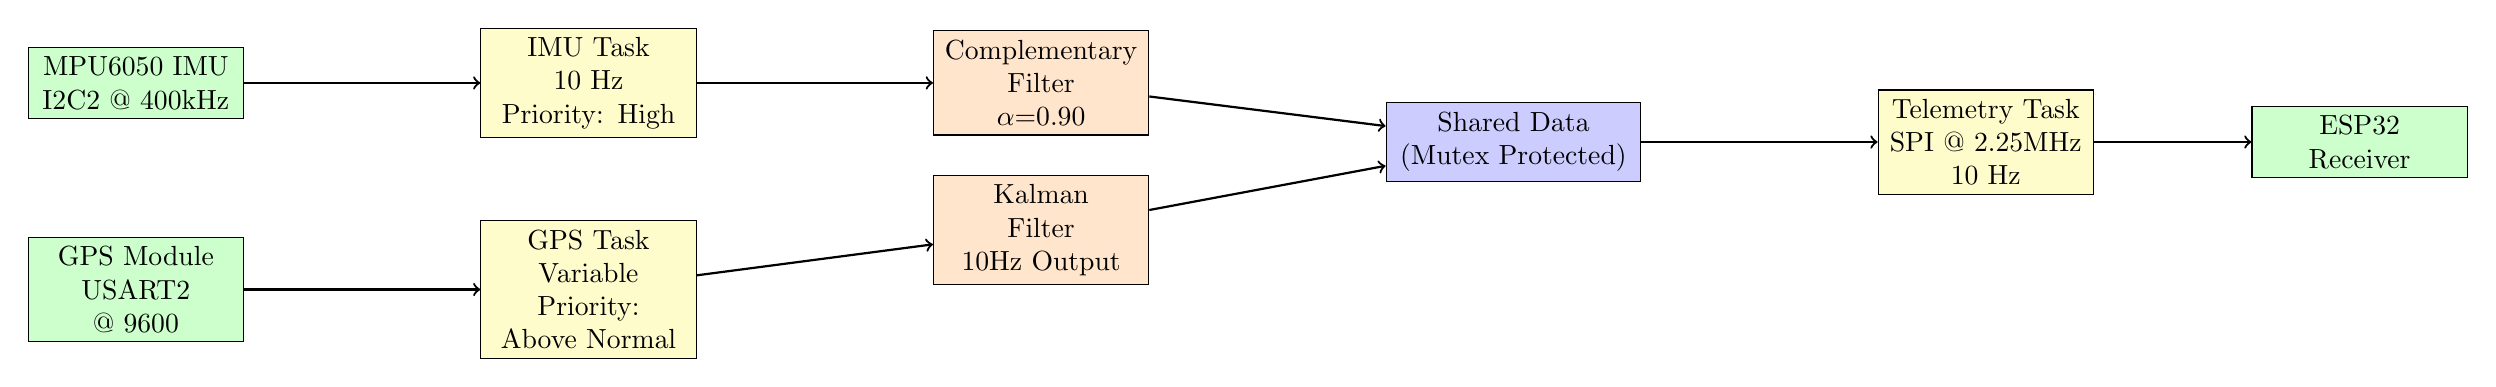
\begin{tikzpicture}[
    node distance=1.5cm,
    box/.style={rectangle, draw, fill=blue!20, text width=3cm, align=center, minimum height=1cm},
    sensor/.style={rectangle, draw, fill=green!20, text width=2.5cm, align=center},
    task/.style={rectangle, draw, fill=yellow!20, text width=2.5cm, align=center},
    filter/.style={rectangle, draw, fill=orange!20, text width=2.5cm, align=center}
]
    % Sensors
    \node[sensor] (mpu) {MPU6050 IMU\\I2C2 @ 400kHz};
    \node[sensor, below=of mpu] (gps) {GPS Module\\USART2 @ 9600};
    
    % Tasks
    \node[task, right=3cm of mpu] (imu_task) {IMU Task\\10 Hz\\Priority: High};
    \node[task, right=3cm of gps] (gps_task) {GPS Task\\Variable\\Priority: Above Normal};
    
    % Filters
    \node[filter, right=3cm of imu_task] (comp) {Complementary\\Filter\\$\alpha$=0.90};
    \node[filter, below=0.5cm of comp] (kalman) {Kalman\\Filter\\10Hz Output};
    
    % Shared Data
    \node[box, right=3cm of comp, yshift=-0.75cm] (shared) {Shared Data\\(Mutex Protected)};
    
    % Output
    \node[task, right=3cm of shared] (tel) {Telemetry Task\\SPI @ 2.25MHz\\10 Hz};
    \node[sensor, right=2cm of tel] (esp) {ESP32\\Receiver};
    
    % Connections
    \draw[->, thick] (mpu) -- (imu_task);
    \draw[->, thick] (gps) -- (gps_task);
    \draw[->, thick] (imu_task) -- (comp);
    \draw[->, thick] (gps_task) -- (kalman);
    \draw[->, thick] (comp) -- (shared);
    \draw[->, thick] (kalman) -- (shared);
    \draw[->, thick] (shared) -- (tel);
    \draw[->, thick] (tel) -- (esp);
\end{tikzpicture}
\caption{Arquitectura de Alto Nivel del Sistema de Telemetría}
\end{figure}

\subsection{Estructura de Tareas FreeRTOS}

El sistema implementa 6 tareas concurrentes con diferentes prioridades:

\begin{table}[H]
\centering
\begin{tabular}{@{}lllll@{}}
\toprule
\textbf{Tarea} & \textbf{Frecuencia} & \textbf{Prioridad} & \textbf{Stack} & \textbf{Función Principal} \\
\midrule
IMU\_Task & 10 Hz & High (3) & 512 words & Lectura MPU6050, filtro complementario \\
GPS\_Task & Variable & Above Normal (2) & 512 words & Parseo NMEA, corrección Kalman \\
Telemetry\_Task & 10 Hz & Above Normal (2) & 512 words & Empaquetado y transmisión SPI \\
UART\_Debug\_Task & 0.5 Hz & Below Normal (1) & 384 words & Salida de depuración \\
LED\_Task & 1 Hz & Low (0) & 128 words & Indicador de latido del sistema \\
Health\_Task & 2 Hz & Low (0) & 256 words & Monitoreo de salud del sistema \\
\bottomrule
\end{tabular}
\caption{Configuración de Tareas FreeRTOS}
\end{table}

\subsection{Flujo de Datos Detallado}

\begin{figure}[H]
\centering
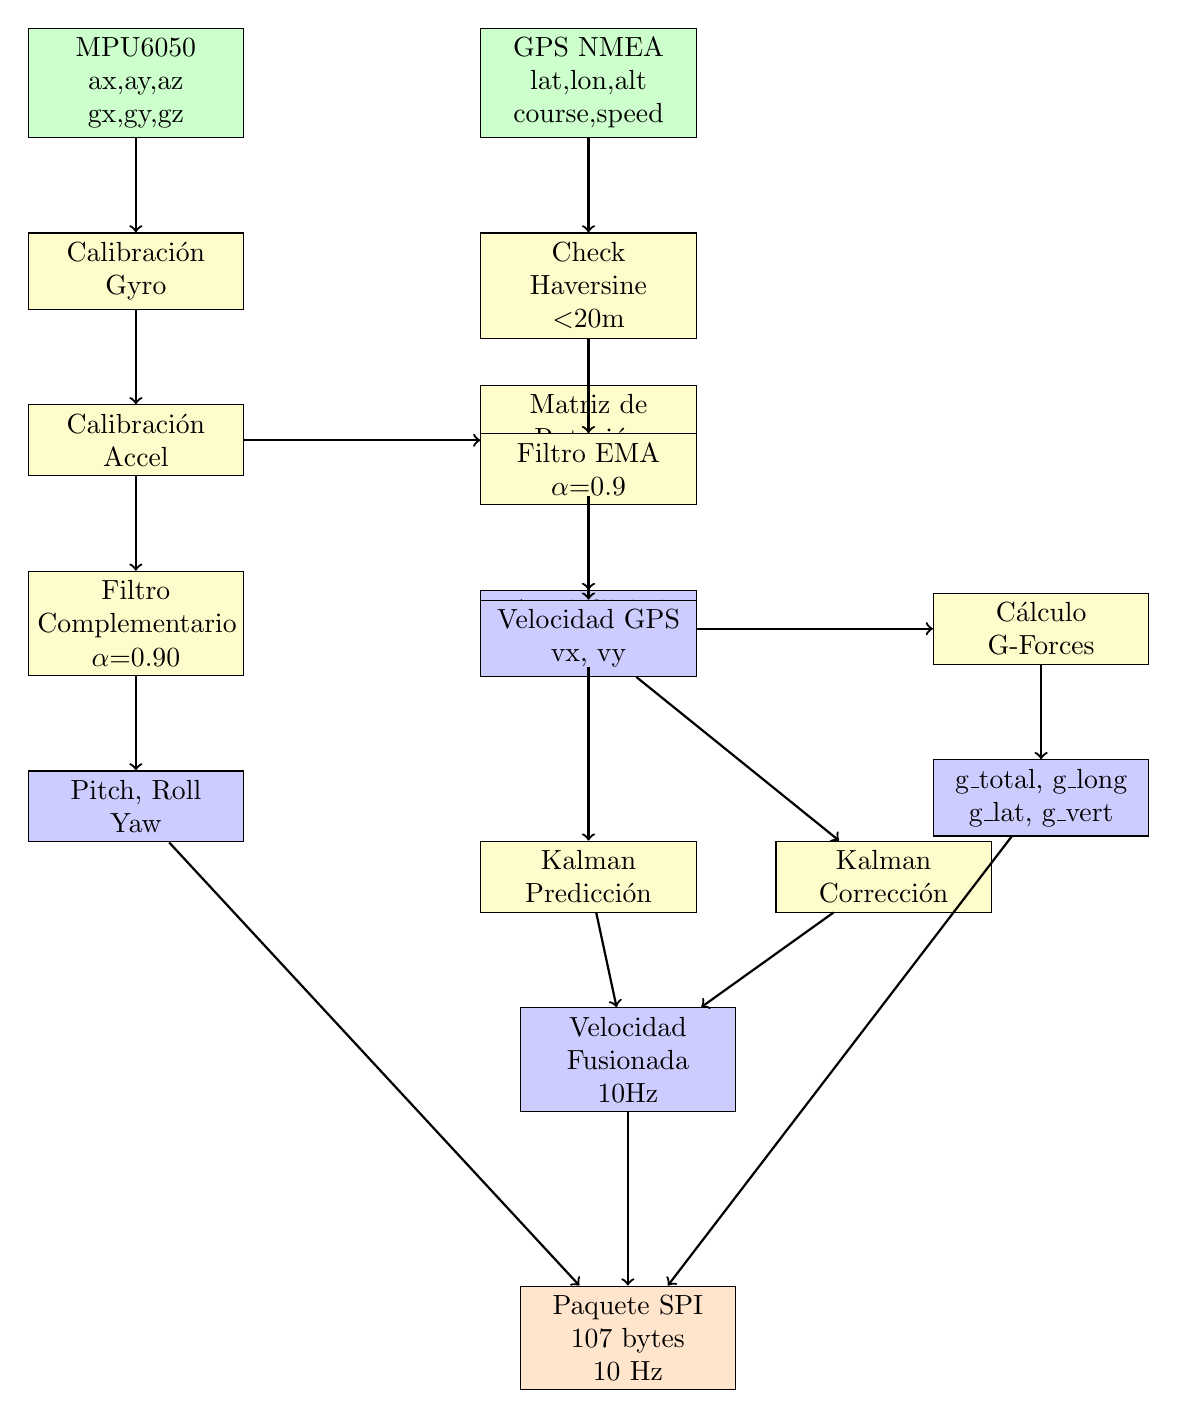
\begin{tikzpicture}[
    node distance=1.2cm,
    box/.style={rectangle, draw, text width=2.5cm, align=center, minimum height=0.8cm},
    process/.style={rectangle, draw, fill=yellow!20, text width=2.5cm, align=center, minimum height=0.8cm}
]
    % IMU Path
    \node[box, fill=green!20] (imu_raw) {MPU6050\\ax,ay,az\\gx,gy,gz};
    \node[process, below=of imu_raw] (gyro_cal) {Calibración\\Gyro};
    \node[process, below=of gyro_cal] (accel_cal) {Calibración\\Accel};
    \node[process, below=of accel_cal] (comp_filt) {Filtro\\Complementario\\$\alpha$=0.90};
    \node[box, fill=blue!20, below=of comp_filt] (angles) {Pitch, Roll\\Yaw};
    
    % Rotation
    \node[process, right=3cm of accel_cal] (rotation) {Matriz de\\Rotación\\Body$\rightarrow$World};
    \node[box, fill=blue!20, below=of rotation] (world_accel) {Accel Global\\wx, wy, wz};
    
    % GPS Path
    \node[box, fill=green!20, right=3cm of imu_raw] (gps_raw) {GPS NMEA\\lat,lon,alt\\course,speed};
    \node[process, below=of gps_raw] (haversine) {Check\\Haversine\\$<$20m};
    \node[process, below=of haversine] (ema) {Filtro EMA\\$\alpha$=0.9};
    \node[box, fill=blue!20, below=of ema] (gps_vel) {Velocidad GPS\\vx, vy};
    
    % Kalman
    \node[process, below=of world_accel, yshift=-1cm] (kalman_p) {Kalman\\Predicción};
    \node[process, right=1cm of kalman_p] (kalman_c) {Kalman\\Corrección};
    \node[box, fill=blue!20, below=of kalman_p, xshift=0.5cm] (fused_vel) {Velocidad\\Fusionada\\10Hz};
    
    % G-Forces
    \node[process, right=3cm of world_accel] (g_calc) {Cálculo\\G-Forces};
    \node[box, fill=blue!20, below=of g_calc] (g_forces) {g\_total, g\_long\\g\_lat, g\_vert};
    
    % Output
    \node[box, fill=orange!20, below=of fused_vel, yshift=-1cm] (telemetry) {Paquete SPI\\107 bytes\\10 Hz};
    
    % Connections
    \draw[->, thick] (imu_raw) -- (gyro_cal);
    \draw[->, thick] (gyro_cal) -- (accel_cal);
    \draw[->, thick] (accel_cal) -- (comp_filt);
    \draw[->, thick] (comp_filt) -- (angles);
    \draw[->, thick] (accel_cal) -- (rotation);
    \draw[->, thick] (rotation) -- (world_accel);
    \draw[->, thick] (gps_raw) -- (haversine);
    \draw[->, thick] (haversine) -- (ema);
    \draw[->, thick] (ema) -- (gps_vel);
    \draw[->, thick] (world_accel) -- (kalman_p);
    \draw[->, thick] (gps_vel) -- (kalman_c);
    \draw[->, thick] (kalman_p) -- (fused_vel);
    \draw[->, thick] (kalman_c) -- (fused_vel);
    \draw[->, thick] (world_accel) -- (g_calc);
    \draw[->, thick] (g_calc) -- (g_forces);
    \draw[->, thick] (angles) -- (telemetry);
    \draw[->, thick] (fused_vel) -- (telemetry);
    \draw[->, thick] (g_forces) -- (telemetry);
\end{tikzpicture}
\caption{Flujo de Procesamiento de Datos desde Sensores hasta Salida}
\end{figure}

\subsection{Estructura del Paquete SPI}

El sistema transmite un paquete de 107 bytes cada 100ms (10Hz) al ESP32:

\begin{table}[H]
\centering
\small
\begin{tabular}{@{}llllp{5cm}@{}}
\toprule
\textbf{Offset} & \textbf{Tamaño} & \textbf{Campo} & \textbf{Tipo} & \textbf{Descripción} \\
\midrule
0 & 1 & Start Byte & uint8 & 0xAA (encabezado) \\
1 & 1 & Packet Type & uint8 & 0x01 (telemetría) \\
2 & 1 & Payload Length & uint8 & 102 bytes \\
\midrule
\multicolumn{5}{c}{\textbf{Orientación (12 bytes)}} \\
\midrule
3-6 & 4 & Pitch & float32 & Ángulo pitch (grados) \\
7-10 & 4 & Roll & float32 & Ángulo roll (grados) \\
11-14 & 4 & Yaw & float32 & Ángulo yaw (grados) \\
\midrule
\multicolumn{5}{c}{\textbf{Tasas (12 bytes)}} \\
\midrule
15-18 & 4 & Pitch Rate & float32 & Tasa pitch (deg/s) \\
19-22 & 4 & Roll Rate & float32 & Tasa roll (deg/s) \\
23-26 & 4 & Yaw Rate & float32 & Tasa yaw (deg/s) \\
\midrule
\multicolumn{5}{c}{\textbf{Aceleración Global (12 bytes)}} \\
\midrule
27-30 & 4 & ax\_global & float32 & Accel Norte/Sur (m/s²) \\
31-34 & 4 & ay\_global & float32 & Accel Este/Oeste (m/s²) \\
35-38 & 4 & az\_global & float32 & Accel Vertical (m/s²) \\
\midrule
\multicolumn{5}{c}{\textbf{Fuerzas G (16 bytes)}} \\
\midrule
39-42 & 4 & g\_total & float32 & Fuerza G total \\
43-46 & 4 & g\_long & float32 & G longitudinal \\
47-50 & 4 & g\_lat & float32 & G lateral \\
51-54 & 4 & g\_vert & float32 & G vertical \\
\midrule
\multicolumn{5}{c}{\textbf{Vibración (4 bytes)}} \\
\midrule
55-58 & 4 & vibration & float32 & Nivel vibración (0-10) \\
\midrule
\multicolumn{5}{c}{\textbf{GPS Básico (20 bytes)}} \\
\midrule
59-62 & 4 & latitude & float32 & Latitud (grados) \\
63-66 & 4 & longitude & float32 & Longitud (grados) \\
67-70 & 4 & altitude & float32 & Altitud (metros) \\
71-74 & 4 & vdop & float32 & DOP Vertical \\
75-78 & 4 & hdop & float32 & DOP Horizontal \\
\midrule
\multicolumn{5}{c}{\textbf{GPS Avanzado (20 bytes)}} \\
\midrule
79-82 & 4 & velocity\_x & float32 & Velocidad Norte (m/s) \\
83-86 & 4 & velocity\_y & float32 & Velocidad Este (m/s) \\
87-90 & 4 & speed & float32 & Velocidad total (m/s) \\
91-94 & 4 & course & float32 & Rumbo (grados) \\
95-98 & 4 & confidence & float32 & Confianza GPS (0-100\%) \\
\midrule
\multicolumn{5}{c}{\textbf{Estado (6 bytes)}} \\
\midrule
99 & 1 & imu\_ok & uint8 & Estado IMU (0/1) \\
100 & 1 & gps\_ok & uint8 & Estado GPS (0/1) \\
101 & 1 & fix & uint8 & Calidad fix GPS (0-2) \\
102 & 1 & state & uint8 & Estado vehículo (0-4) \\
103 & 1 & confidence & uint8 & Confianza sistema \\
104 & 1 & wheel\_contact & uint8 & Máscara contacto ruedas \\
\midrule
\multicolumn{5}{c}{\textbf{Footer (3 bytes)}} \\
\midrule
105 & 1 & Checksum & uint8 & XOR de bytes 0-104 \\
106 & 1 & End Byte & uint8 & 0x55 (pie de paquete) \\
\bottomrule
\end{tabular}
\caption{Estructura Completa del Paquete de Telemetría SPI}
\end{table}

\subsection{Algoritmos Clave}

\subsubsection{Filtro Complementario}

El filtro complementario combina giroscopio (rápido, deriva) con acelerómetro (lento, ruidoso):

\begin{equation}
\theta_{filtrado} = \alpha \cdot (\theta_{anterior} + \omega \cdot \Delta t) + (1-\alpha) \cdot \theta_{accel}
\end{equation}

Donde:
\begin{itemize}
    \item $\alpha = 0.90$ (90\% giroscopio, 10\% acelerómetro)
    \item $\omega$ = Tasa angular del giroscopio (deg/s)
    \item $\Delta t$ = Paso de tiempo (0.1s @ 10Hz)
    \item $\theta_{accel}$ = Ángulo del acelerómetro
\end{itemize}

\textbf{Ventajas}:
\begin{itemize}
    \item Respuesta rápida del giroscopio para movimientos dinámicos
    \item Corrección de deriva del acelerómetro a largo plazo
    \item Computacionalmente eficiente (sin inversión de matrices)
\end{itemize}

\subsubsection{Filtro de Kalman para Velocidad}

El filtro de Kalman fusiona GPS (1Hz, preciso) con IMU (10Hz, rápido):

\paragraph{Paso de Predicción (10Hz, IMU):}
\begin{align}
v_{pred} &= v_{anterior} + a \cdot \Delta t \\
P_{pred} &= P_{anterior} + Q
\end{align}

\paragraph{Paso de Corrección (1Hz, GPS):}
\begin{align}
K &= \frac{P_{pred}}{P_{pred} + R} \quad \text{(Ganancia de Kalman)} \\
v_{corr} &= v_{pred} + K \cdot (v_{GPS} - v_{pred}) \\
P_{corr} &= (1 - K) \cdot P_{pred}
\end{align}

Donde:
\begin{itemize}
    \item $Q = 0.05$ (ruido del proceso - confianza IMU)
    \item $R_{GPS} = 1.0$ (ruido de medición GPS)
    \item $R_{IMU} = 0.2$ (ruido de medición IMU)
\end{itemize}

\textbf{Resultado}: Salida de velocidad suave a 10Hz con corrección de deriva GPS cada segundo.

\subsubsection{Matriz de Rotación (Body $\rightarrow$ World)}

Para integrar correctamente la aceleración en velocidad, se debe transformar del marco del sensor al marco mundial:

\begin{align}
w_x &= c_y(c_p \cdot a_x + s_p s_r \cdot a_y + s_p c_r \cdot a_z) - s_y(c_r \cdot a_y - s_r \cdot a_z) \\
w_y &= s_y(c_p \cdot a_x + s_p s_r \cdot a_y + s_p c_r \cdot a_z) + c_y(c_r \cdot a_y - s_r \cdot a_z) \\
w_z &= -s_p \cdot a_x + c_p s_r \cdot a_y + c_p c_r \cdot a_z
\end{align}

Donde: $c_p = \cos(pitch)$, $s_p = \sin(pitch)$, etc.

\subsubsection{Filtrado de Datos GPS}

\paragraph{Verificación de Distancia Haversine:}
Rechaza saltos GPS $>$ 20m entre lecturas consecutivas para prevenir valores atípicos.

\paragraph{Filtro EMA (Exponential Moving Average):}
\begin{align}
lat_{filtrado} &= 0.9 \cdot lat_{anterior} + 0.1 \cdot lat_{nuevo} \\
lon_{filtrado} &= 0.9 \cdot lon_{anterior} + 0.1 \cdot lon_{nuevo}
\end{align}

Suaviza el ruido de posición GPS manteniendo capacidad de respuesta.

\paragraph{Fusión de Yaw:}
Cuando velocidad $>$ 1 m/s, el rumbo GPS corrige la deriva del yaw del IMU.

\subsection{Análisis de Temporización y Rendimiento}

\begin{table}[H]
\centering
\begin{tabular}{@{}lllll@{}}
\toprule
\textbf{Tarea} & \textbf{Frecuencia} & \textbf{Período} & \textbf{Tiempo CPU} & \textbf{Margen} \\
\midrule
IMU\_Task & 10 Hz & 100 ms & $\sim$15 ms & 85\% \\
GPS\_Task & $\sim$1 Hz & 1000 ms & $\sim$5 ms & 99.5\% \\
Telemetry\_Task & 10 Hz & 100 ms & $\sim$8 ms & 92\% \\
UART\_Debug\_Task & 0.5 Hz & 2000 ms & $\sim$10 ms & 99.5\% \\
LED\_Task & 1 Hz & 1000 ms & $<$1 ms & 99.9\% \\
Health\_Task & 2 Hz & 500 ms & $\sim$2 ms & 99.6\% \\
\bottomrule
\end{tabular}
\caption{Análisis de Temporización de Tareas}
\end{table}

\textbf{Utilización Total de CPU}: $\sim$15\% (amplio margen para expansión futura)

\subsection{Protocolos de Comunicación}

\subsubsection{I2C2 (MPU6050)}
\begin{itemize}
    \item \textbf{Velocidad}: 400 kHz (Modo Rápido)
    \item \textbf{Pines}: PB10 (SCL), PB11 (SDA)
    \item \textbf{Pull-ups}: Externos 4.7k$\Omega$ requeridos
    \item \textbf{Dirección}: 0x68 (7-bit)
    \item \textbf{Timeout}: 200 ms
\end{itemize}

\subsubsection{SPI2 (ESP32)}
\begin{itemize}
    \item \textbf{Velocidad}: 2.25 MHz
    \item \textbf{Modo}: Modo 0 (CPOL=0, CPHA=0)
    \item \textbf{Pines}: PB13 (SCK), PC3 (MOSI), PC2 (MISO), PB12 (CS)
    \item \textbf{CS}: Activo BAJO, controlado por GPIO
    \item \textbf{Timeout}: 100 ms
\end{itemize}

\subsubsection{USART2 (GPS)}
\begin{itemize}
    \item \textbf{Baud}: 9600
    \item \textbf{Pines}: PA3 (RX), PA2 (TX - sin usar)
    \item \textbf{DMA}: Modo circular en RX
    \item \textbf{Protocolo}: NMEA 0183 (\$GNGGA, \$GNRMC)
\end{itemize}

\subsubsection{USART3 (Debug)}
\begin{itemize}
    \item \textbf{Baud}: 115200
    \item \textbf{Pines}: PD8 (TX), PD9 (RX - sin usar)
    \item \textbf{Formato}: Telemetría legible para humanos
\end{itemize}

\subsection{Manejo de Errores y Tolerancia a Fallos}

\subsubsection{Reintentos de Inicialización}
\begin{itemize}
    \item Inicialización MPU6050: Hasta 3 reintentos con retardo de 500ms
    \item Verificación WHO\_AM\_I (debe ser 0x68)
    \item Escaneo de bus I2C al inicio para diagnóstico
\end{itemize}

\subsubsection{Sistema Watchdog}
\begin{itemize}
    \item Watchdog de tareas monitorea todas las tareas críticas
    \item Timeout: 5 segundos por tarea
    \item Las tareas deben llamar \texttt{TaskWatchdog\_Feed()} regularmente
\end{itemize}

\subsubsection{Degradación Elegante}
\begin{itemize}
    \item El sistema continúa si falla GPS (modo solo IMU)
    \item El sistema continúa si falla IMU (modo solo GPS)
    \item La tarea Health monitorea frescura de datos (2s para IMU, 5s para GPS)
\end{itemize}

\subsubsection{Códigos de Diagnóstico LED}
\begin{itemize}
    \item \textbf{3x Parpadeo Rápido}: Alcanzó main()
    \item \textbf{2x Parpadeo}: HAL inicializado
    \item \textbf{1x Parpadeo Largo}: Reloj configurado
    \item \textbf{5x Parpadeo (200ms)}: Periféricos inicializados
    \item \textbf{Latido 1 Hz}: FreeRTOS ejecutándose normalmente
    \item \textbf{Parpadeo Rápido (100ms)}: Error\_Handler activado
\end{itemize}

\subsection{Resumen del Sistema}

Este sistema de telemetría es un \textbf{sistema embebido en tiempo real listo para producción} que presenta:

\begin{itemize}
    \item ✓ \textbf{Fusión multi-sensor} (IMU + GPS)
    \item ✓ \textbf{Filtrado avanzado} (Complementario + Kalman)
    \item ✓ \textbf{Telemetría de alta velocidad} (10Hz SPI a ESP32)
    \item ✓ \textbf{Tolerancia a fallos} (watchdog, reintentos, degradación elegante)
    \item ✓ \textbf{Diagnóstico completo} (UART debug, USB CDC, códigos LED)
    \item ✓ \textbf{Rendimiento optimizado} (Planificación basada en prioridades FreeRTOS)
\end{itemize}

El sistema proporciona \textbf{orientación precisa, velocidad, fuerzas G y estado del vehículo} para monitoreo en tiempo real y registro de datos en un entorno de carreras Baja.

\end{document}

